%!LW recipe=latexmk-xelatex
\documentclass[compress]{beamer}

\usetheme[block=fill]{metropolis}

\usepackage{graphicx} % Allows including images
\usepackage{amsmath,amsfonts,amsthm,amssymb}
\usepackage{color}
\usepackage{xcolor,cancel}
\definecolor{mDarkBrown}{HTML}{604c38}
\definecolor{mDarkTeal}{HTML}{23373b}
\definecolor{mLightBrown}{HTML}{EB811B}
\definecolor{mMediumBrown}{HTML}{C87A2F}
\definecolor{mygreen}{HTML}{98C2B9}
\definecolor{myyellow}{HTML}{DFD79C}
\definecolor{myblue}{HTML}{8CA7CC}
\definecolor{kern}{HTML}{8CC2B7}


\usepackage{float}
\usepackage{framed}
\usepackage{epsfig}
\usepackage{graphicx}
\usepackage{subcaption}
\usepackage{ulem}
\usepackage{hhline}
\usepackage{multirow}
\usepackage{multicol}
\usepackage{comment}   
\usepackage{bbm}
\usepackage{tikz}   
\def\Put(#1,#2)#3{\leavevmode\makebox(0,0){\put(#1,#2){#3}}}
\newcommand*\mystrut[1]{\vrule width0pt height0pt depth#1\relax}
\newcommand{\eqdef}{\mathbin{\stackrel{\rm def}{=}}}


\newcommand{\bs}[1]{\boldsymbol{#1}}
\newcommand{\bv}[1]{\mathbf{#1}}
\newcommand{\R}{\mathbb{R}}
\newcommand{\E}{\mathbb{E}}

\DeclareMathOperator*{\argmin}{arg\,min}
\DeclareMathOperator*{\argmax}{arg\,max}
\DeclareMathOperator{\nnz}{nnz}
\DeclareMathOperator{\Var}{Var}
\DeclareMathOperator{\sinc}{sinc}
\DeclareMathOperator{\sign}{sign}
\DeclareMathOperator{\dist}{dist}
\DeclareMathOperator{\mv}{mv}
\DeclareMathOperator{\sgn}{sgn}
\DeclareMathOperator{\step}{step}
\DeclareMathOperator{\gap}{gap}
\DeclareMathOperator{\poly}{poly}
\DeclareMathOperator{\tr}{tr}
\DeclareMathOperator{\orth}{orth}
\newcommand{\norm}[1]{\|#1\|}
\captionsetup[subfigure]{labelformat=empty}
\captionsetup[figure]{labelformat=empty}
\DeclareMathOperator*{\lmin}{\lambda_{min}}
\DeclareMathOperator*{\lmax}{\lambda_{max}}

\newcommand{\specialcell}[2][c]{%
  \begin{tabular}[#1]{@{}c@{}}#2\end{tabular}}
\newcommand{\specialcellleft}[2][c]{%
\begin{tabular}[#1]{@{}l@{}}#2\end{tabular}
}

\usepackage{tabstackengine}
\stackMath


%----------------------------------------------------------------------------------------
%	TITLE PAGE
%----------------------------------------------------------------------------------------

\title{CS-GY 6763: Lecture 6 \\ Near-neighbor search in high dimensions}
\author{NYU Tandon School of Engineering, Prof. Christopher Musco}
\date{}

\begin{document}

\begin{frame}
	\titlepage 
\end{frame}

\metroset{titleformat=smallcaps}


\begin{frame}
	\frametitle{last class}
	\textbf{Dimensionality reduction:} Given vectors $\bv{x}, \bv{y}$, compute small space compressions $C(\bv{x})$ and $C(\bv{y})$ that can be used to estimate the distance or similarity between $\bv{x}$ and $\bv{y}$. 
\end{frame}

\begin{frame}
	\frametitle{euclidean dimensionality reduction}
	\begin{lemma}[Distributional JL Lemma]
		Let $\bs{\Pi}$ be a random matrix that compresses to $k = O\left(\frac{\log(1/\delta)}{\epsilon^2}\right)$ rows. Then with probability $(1-\delta)$:
		\begin{align*}
			(1-\epsilon)\|\bv{x} - \bv{y}\|_2^2 \leq \|\bs{\Pi}\bv{x} - \bs{\Pi}\bv{y}\|_2^2 \leq (1+\epsilon) \|\bv{x} - \bv{y}\|_2^2
		\end{align*}
	\end{lemma}
	
	\begin{center}
		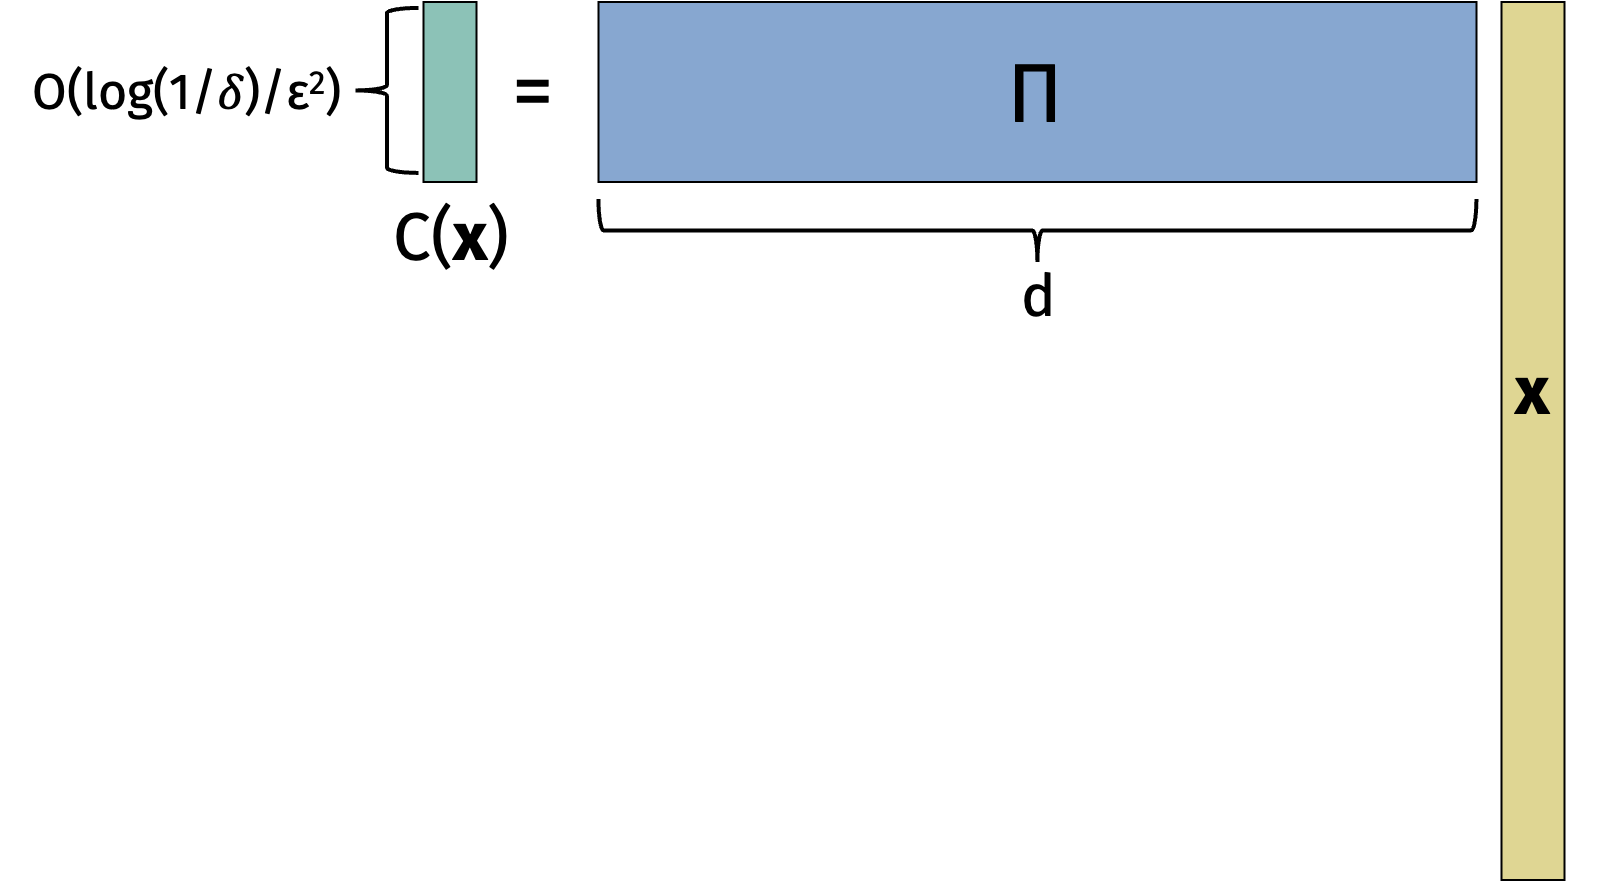
\includegraphics[height=.55\textheight]{jl_refresh.png}
	\end{center}
\end{frame}

\begin{frame}
	\frametitle{dimensionality reduction for jaccard similarity}
	\begin{lemma}[MinHash]
		Let $C$ be a length $k = O\left(\frac{\log(1/\delta)}{\epsilon^2}\right)$ MinHash sketch. Then with probability $(1-\delta)$, we can return an estimate $\tilde{J}$ based on $C(\bv{x})$ and $C(\bv{y})$ with:
		\begin{align*}
			J(\bv{x},\bv{y}) - \epsilon \leq \tilde{J} \leq J(\bv{x},\bv{y}) + \epsilon.	
		\end{align*}
	\end{lemma}
	
	\begin{center}
		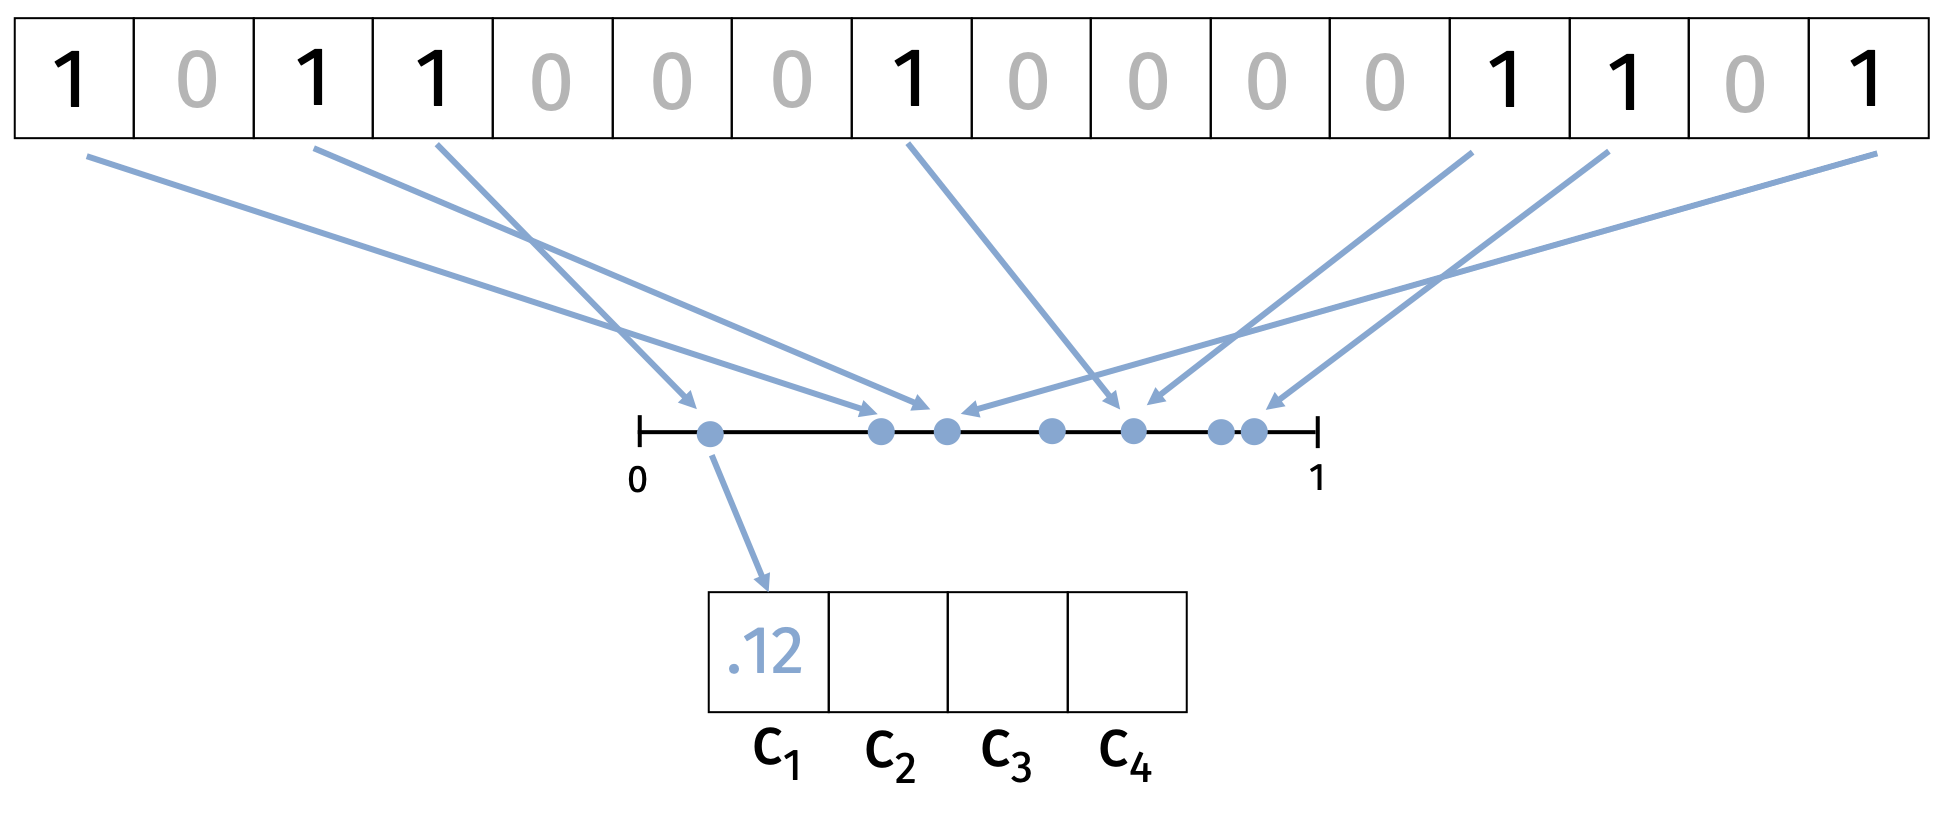
\includegraphics[width=.8\textwidth]{minHash1.png}	
	\end{center}
\end{frame}

\begin{frame}
	\frametitle{key application: modern vector sea search}
	\begin{center}
		\vspace{-.5em}
				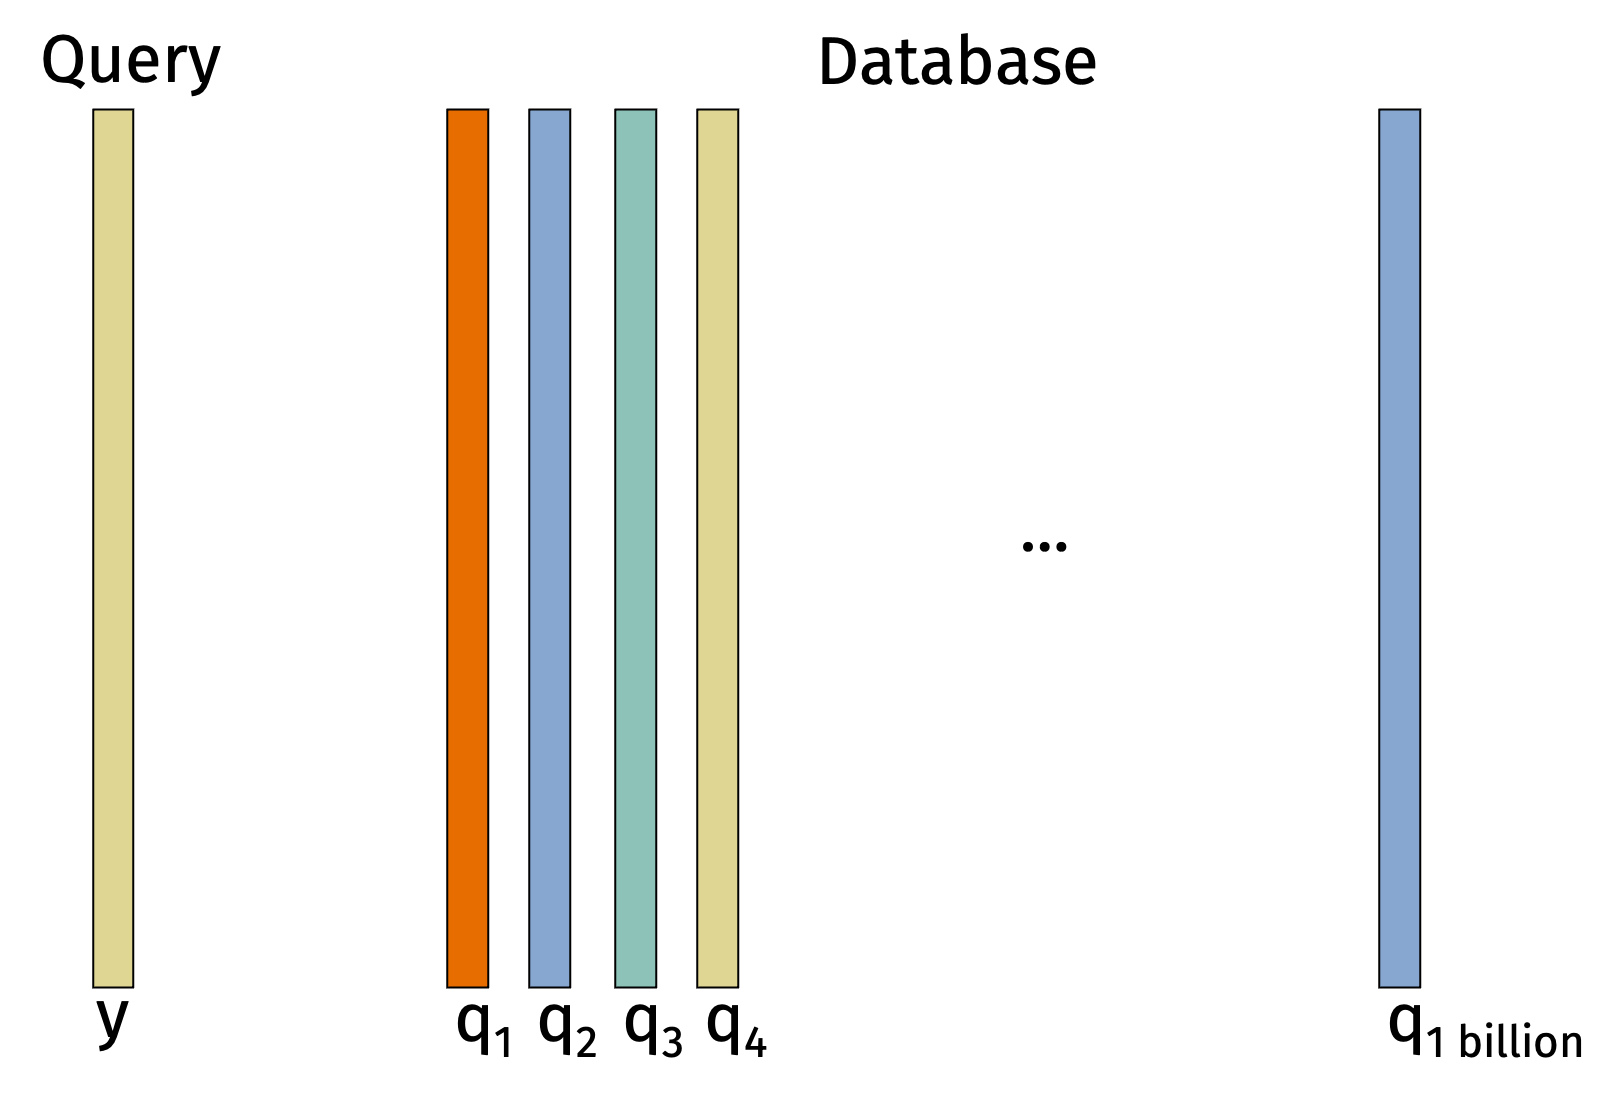
\includegraphics[width=.8\textwidth]{vector_search_recap.png}
				\vspace{-.5em}
	\end{center}
	Cost of naive algorithm is $O(nd)$. 
\end{frame}

\begin{frame}
	\frametitle{key application: modern vector sea search}
	Dimensionality reduction reduces search cost to $O(nk)$ and reduces space requirements.
	\begin{center}
		\vspace{-.5em}
				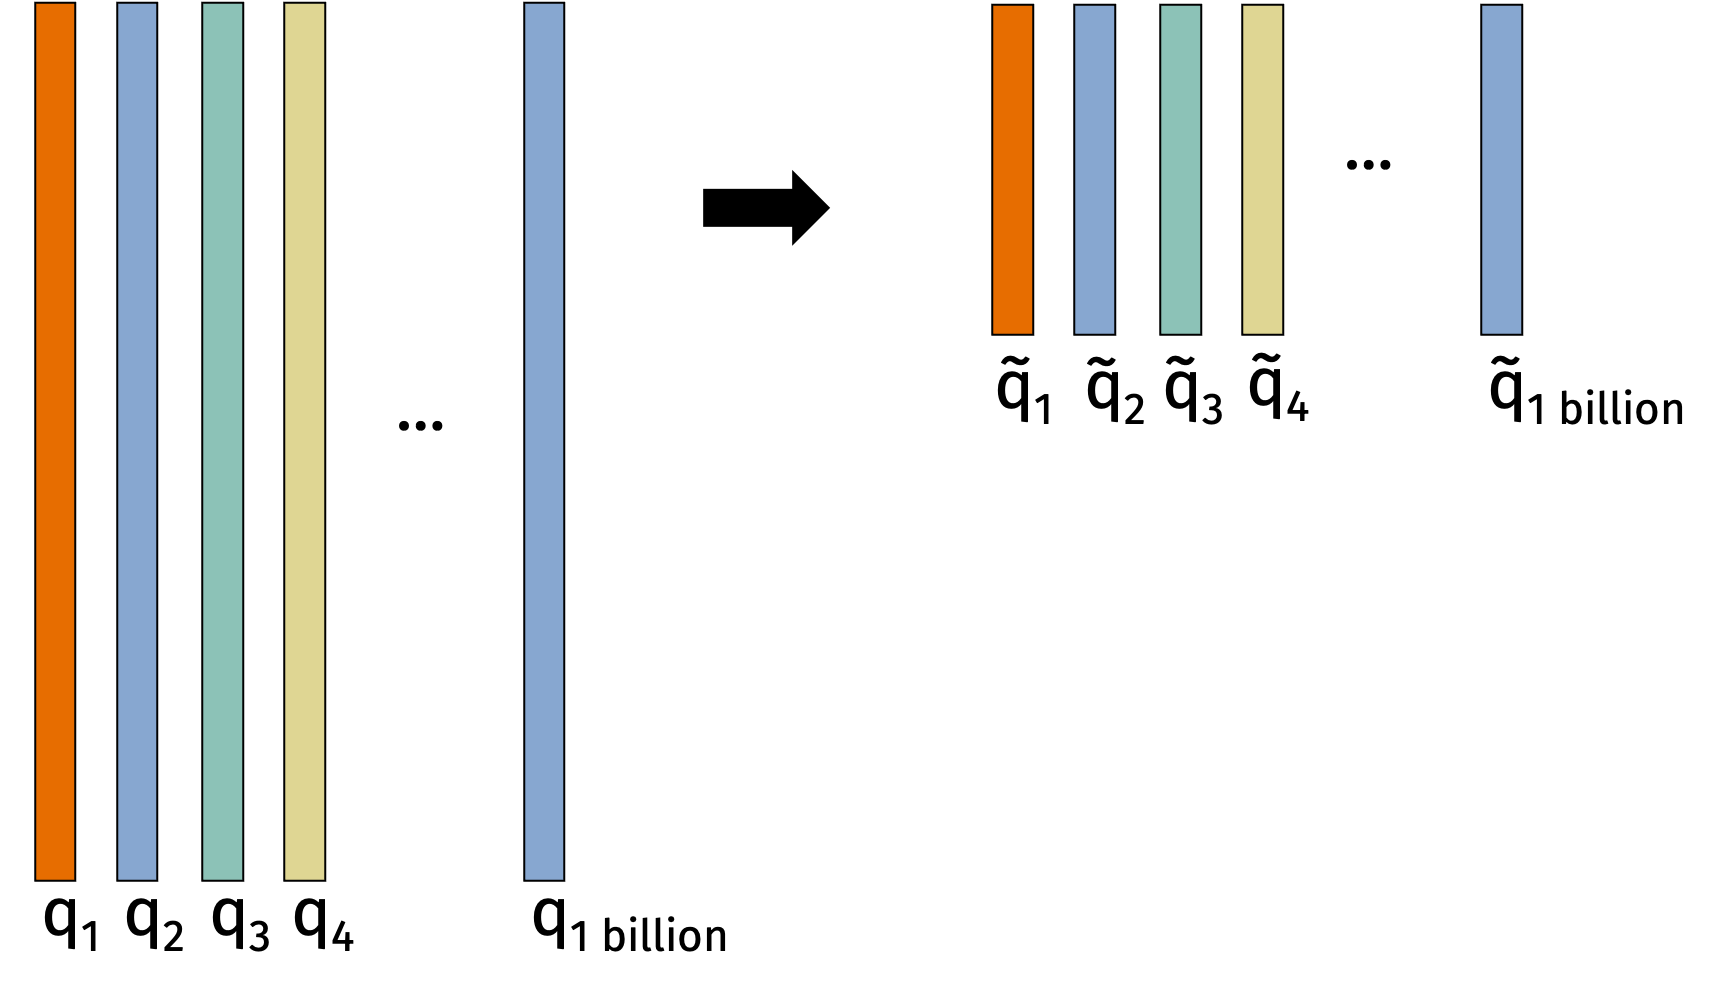
\includegraphics[width=.7\textwidth]{vector_search_recap2.png}
				\vspace{-.75em}
	\end{center}
	 All modern vector search systems use ``fancier'' versions of methods studied in this class:
	 \vspace{-.25em}
	 \begin{multicols}{2}
		\begin{itemize}
			\item Quantized JL/SimHash
			\item b-bit MinHash
			\item Product Quantization 
			\item PCA-based methods
		\end{itemize}
		\end{multicols}
\end{frame} 

\begin{frame}
	\frametitle{vector indexing / near neighbor search}
	Dimensionality reduction methods are typically paired with \emph{vector indexing methods}.

	\textbf{Goal of Dimensionality Reduction:} Reduce \alert{\textbf{dependence on $d$}} in $O(nd)$ search cost. Reduce space complexity. 

	\textbf{Goal of Vector Indexing:} Reduce \alert{\textbf{dependence on $n$}} in $O(nd)$ search cost. Often at the cost of added space complexity. 
\end{frame}

\begin{frame}
	\frametitle{beyond a linear scan}	
	This problem can already be solved in low-dimensions using space partitioning approaches (namely, kd-trees).
	
	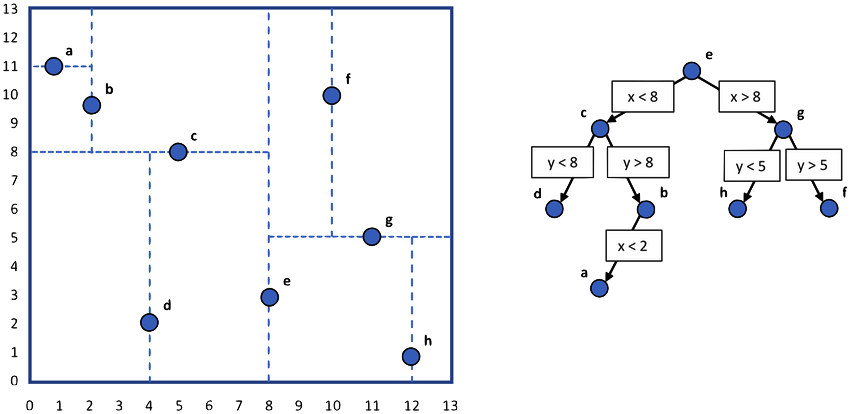
\includegraphics[height=.4\textheight]{kdtree.png}	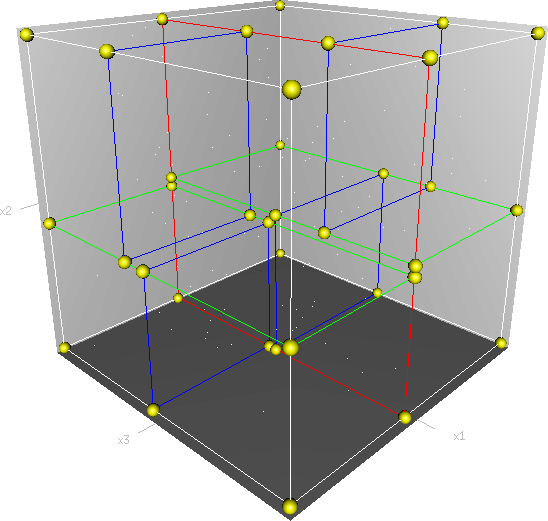
\includegraphics[height=.4\textheight]{3dtree.png}
	
	Search time is roughly $O(d\cdot  \log n \cdot 2^d))$, which is only sublinear for $d = o(\log n)$.
\end{frame}

\begin{frame}
	\frametitle{issue with kd-trees}	

	
	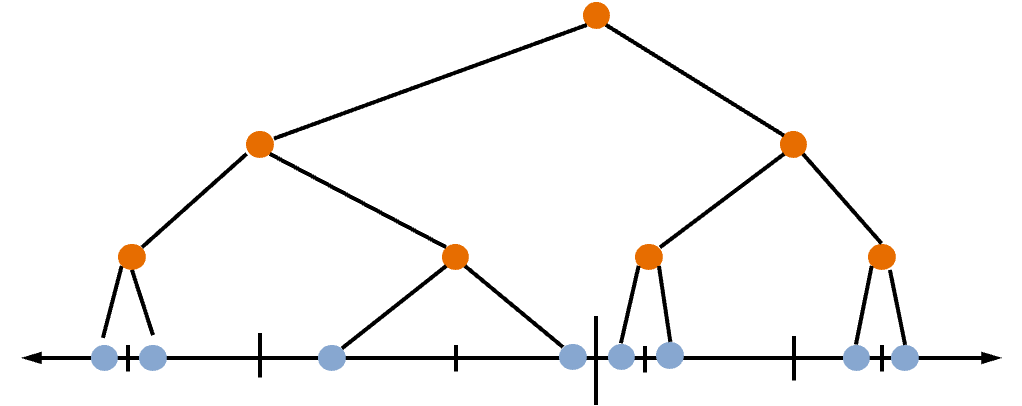
\includegraphics[width=\textwidth]{1d-kd_tree.png}	
\end{frame}

\begin{frame}
	\frametitle{issue with kd-trees}	
	\vspace{1em}

	\centering
	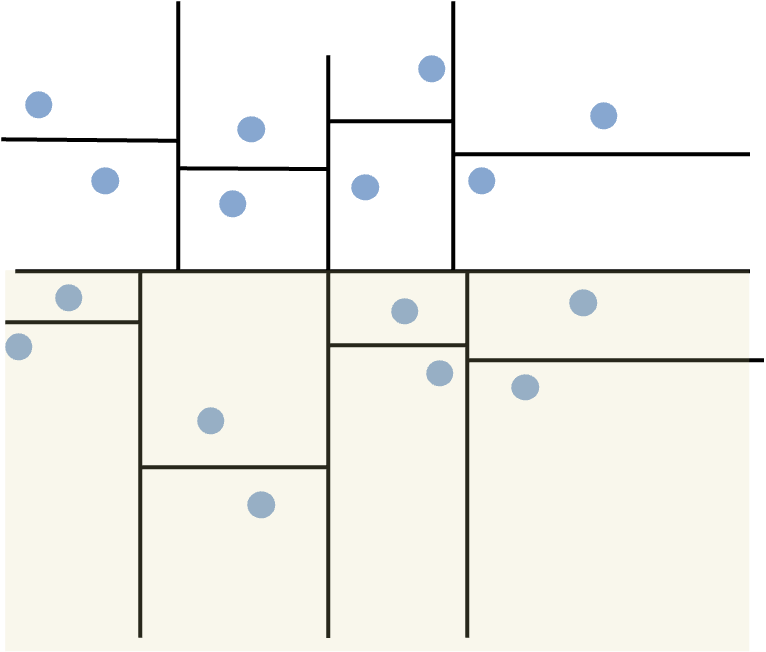
\includegraphics[width=.8\textwidth]{2d-kd-tree.png}	
\end{frame}

\begin{frame}
	\frametitle{high dimensional near neighbor search}	
	Only been attacked much more recently:
	\begin{itemize}
		\item \textbf{\alert{Locality-sensitive hashing [Indyk, Motwani, 1998]}}
		\item Spectral hashing [Weiss, Torralba, and Fergus, 2008]
		\item Vector quantization [J\'{e}gou, Douze, Schmid, 2009]
		\item Graph-based vector search [Malkov, Yashunin, 2016, Subramanya et al., 2019]
	\end{itemize}

\textbf{Key ideas behind all of these methods:} 
\begin{enumerate}
\item Trade worse space-complexity + preprocessing time for better time-complexity. I.e., preprocess database in data structure that uses $\Omega(n)$ space.
\item Allow for approximation.
\end{enumerate}
\end{frame}

\begin{frame}[t]
	\frametitle{intuitively why do preprocessing and space help?}	
	\textbf{Question:} Suppose you want to search over points in $[-1,1]^d$ and to achieve accuracy $\epsilon$. I.e., for a given $\bv{y}\in [-1,1]^d$, you want to find $\tilde{\bv{q}}$ with $\|\bv{y} - \tilde{\bv{q}}\|_2 \leq \min_{i}\|\bv{y} - \bv{q}_i\|_2 + \epsilon$. 
	
	Can you construct a data structure that supports $O(1)$ time search but uses \emph{exponential space}?

\end{frame}

\begin{frame}
	\frametitle{locality sensitive hash functions}
	Let $h: \R^d \rightarrow \{1, \ldots, m\}$ be a random hash function. 
	
	We call $h$ \emph{locality sensitive} for similarity function $s(\bv{q},\bv{y})$ if $\Pr\left[h(\bv{q}) == h(\bv{y})\right]$ is:
	\begin{itemize}
		\item Higher when $\bv{q}$ and $\bv{y}$ are more similar, i.e. $s(\bv{q},\bv{y})$ is higher.
		\item Lower when $\bv{q}$ and $\bv{y}$ are more dissimilar, i.e. $s(\bv{q},\bv{y})$ is lower. 
	\end{itemize}
\begin{center}
	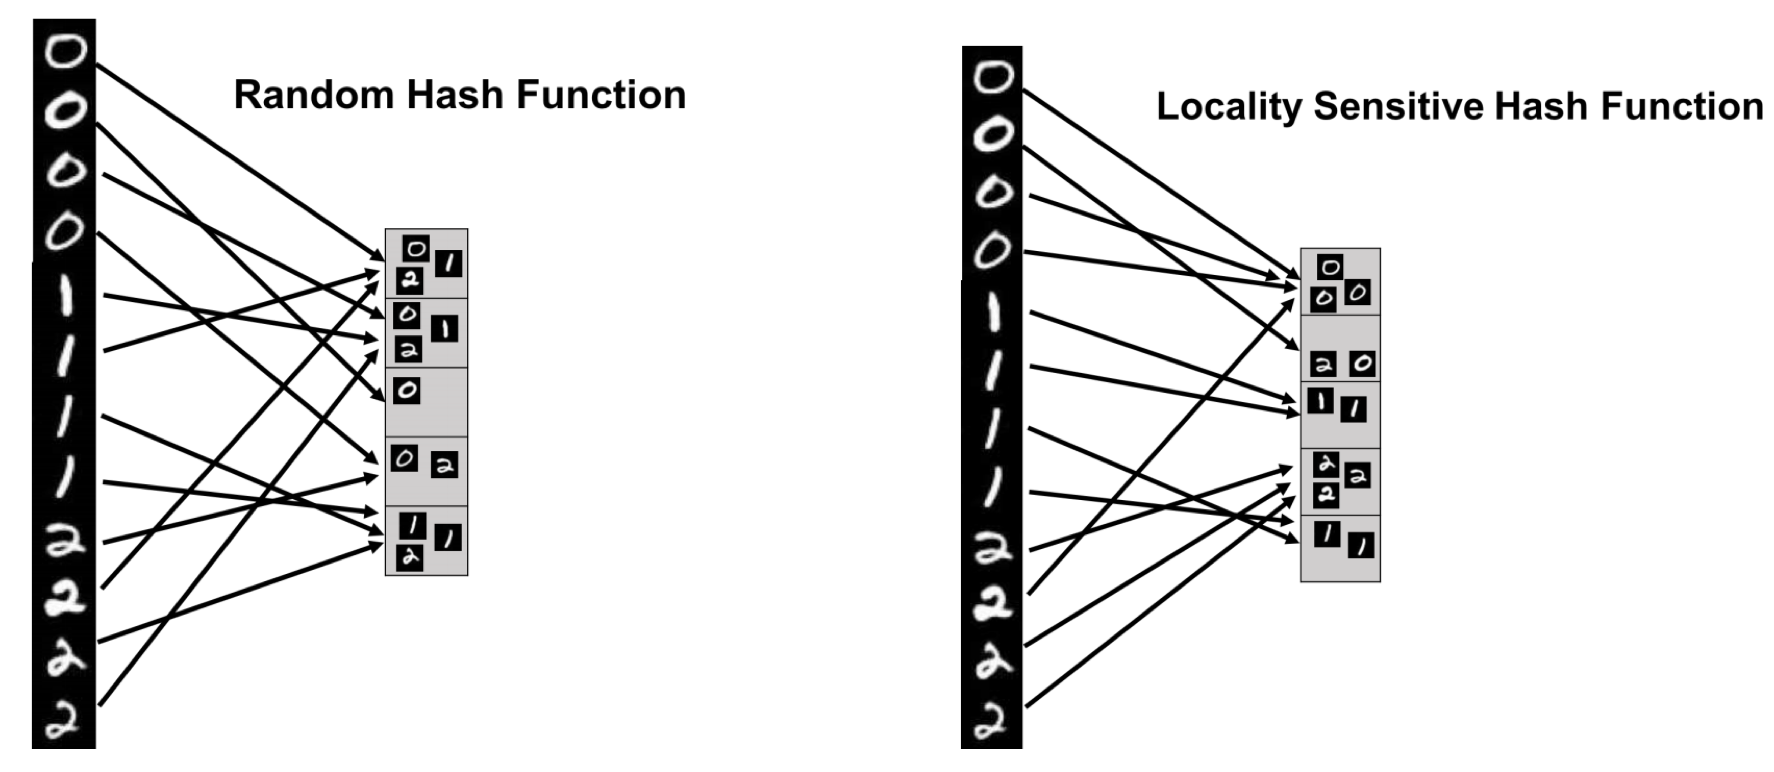
\includegraphics[width=.9\textwidth]{cam_lsh.png}
\end{center}
\end{frame}

\begin{frame}
	\frametitle{locality sensitive hash functions}
	LSH for $s(\bv{q},\bv{y})$  equal to Jaccard similarity:
	\begin{itemize}
		\item Let $c: \{0,1\}^d \rightarrow [0,1]$ be a single instantiation of MinHash.
		\item Let $g: [0,1] \rightarrow \{1, \ldots, m\}$ be a uniform random hash function.
		\item Let $h(\bv{q}) = g(c(\bv{q})).$
	\end{itemize}
\begin{center}
	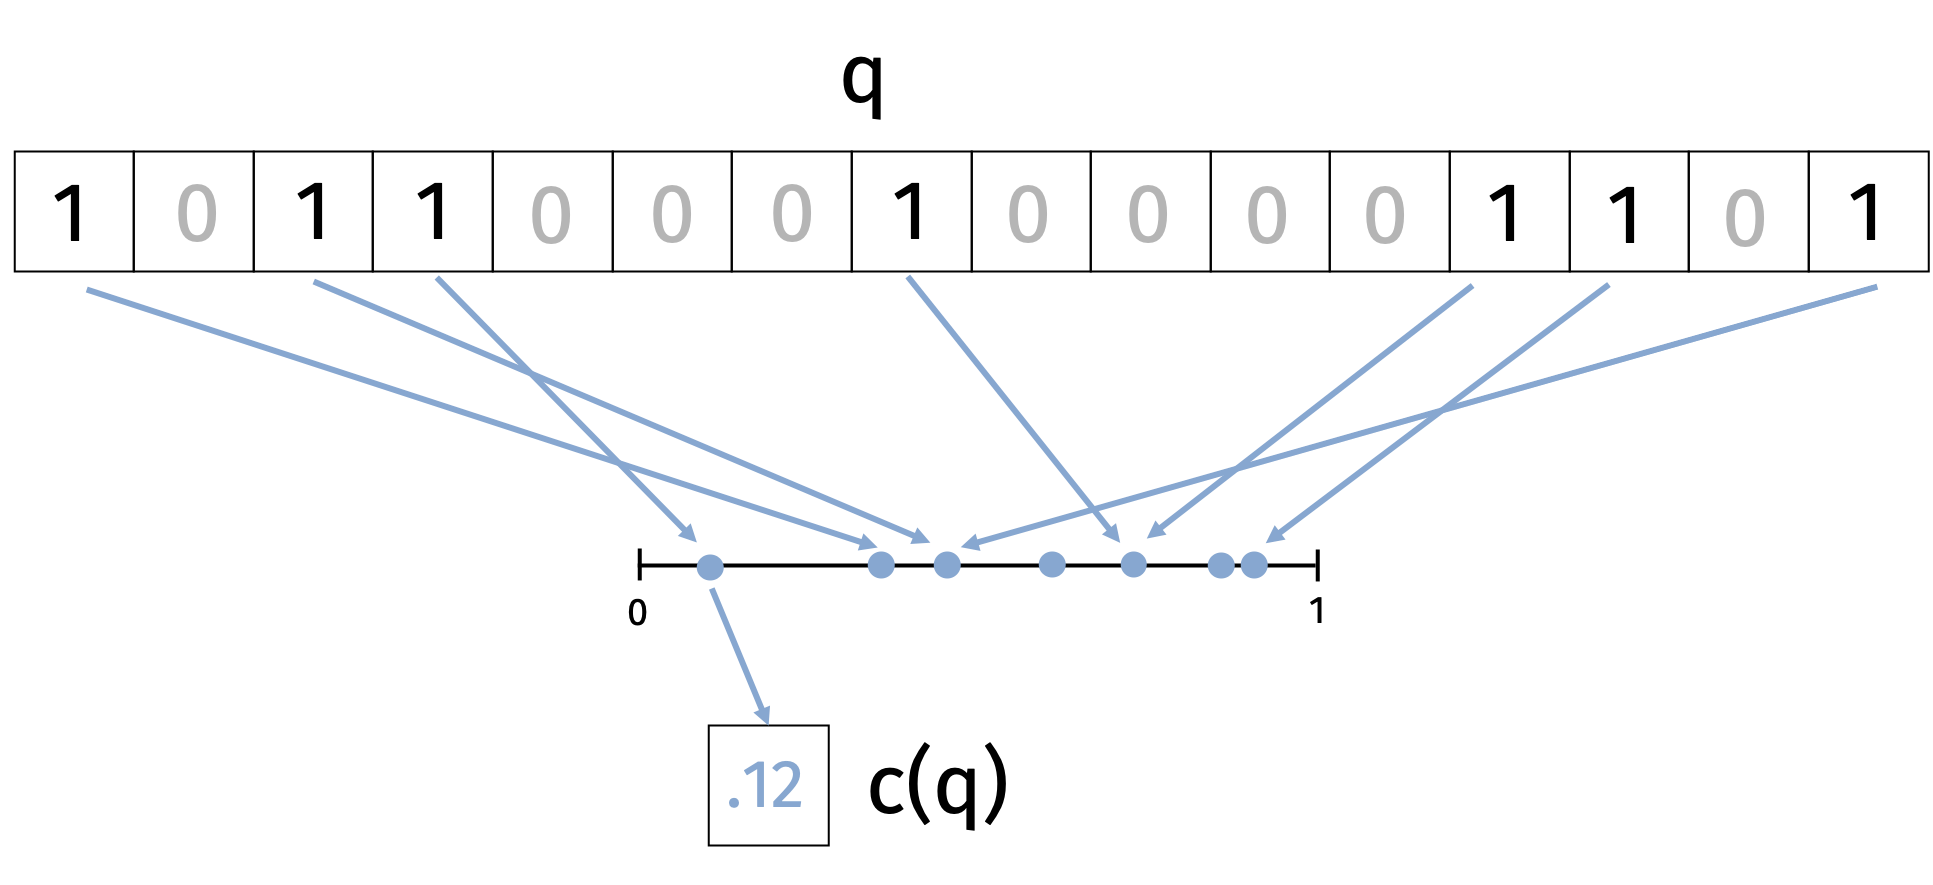
\includegraphics[width=.7\textwidth]{single_min_hash.png}
\end{center}

\end{frame}

\begin{frame}
	\frametitle{locality sensitive hash functions}
	LSH for Jaccard similarity:
	\begin{itemize}
		\item Let $c: \{0,1\}^d \rightarrow [0,1]$ be a single instantiation of MinHash.
		\item Let $g: [0,1] \rightarrow \{1, \ldots, m\}$ be a uniform random hash function.
		\item Let $h(\bv{x}) = g(c(\bv{x})).$
	\end{itemize}
		If $J(\bv{q},\bv{y}) = v$, 
		\begin{align*}
			\Pr\left[h(\bv{q}) == h(\bv{y})\right] = \hspace{15em}
		\end{align*}
\end{frame}

\begin{frame}
	\frametitle{near neighbor search}
	\begin{center}
	Basic approach for LSH-based near neighbor search in a database.
	\end{center}
		\textbf{Pre-processing:}
	\begin{itemize}
		\item Select random LSH function $h: \{0,1\}^d \rightarrow 1,\ldots, m$.
		\item Create table $T$ with $m = O(n)$ slots.\footnote{Enough to make the $O(1/m)$ term negligible.}
		\item For $i = 1,\ldots, n$, insert $\bv{q}_i$ into $T(h(\bv{q}_i))$.
	\end{itemize}
	\textbf{Query:}
	\begin{itemize}
		\item Want to find near neighbors of input $\bv{y}\in\{0,1\}^d$.
		\item Linear scan through all vectors $\bv{q}\in T(h(\bv{y}))$ and return any that are close to $\bv{y}$. Time required is $O(d\cdot |T(h(\bv{y})|)$.
	\end{itemize}
\vspace{1em}
\end{frame}

\begin{frame}
	\frametitle{near neighbor search}
	\begin{center}
		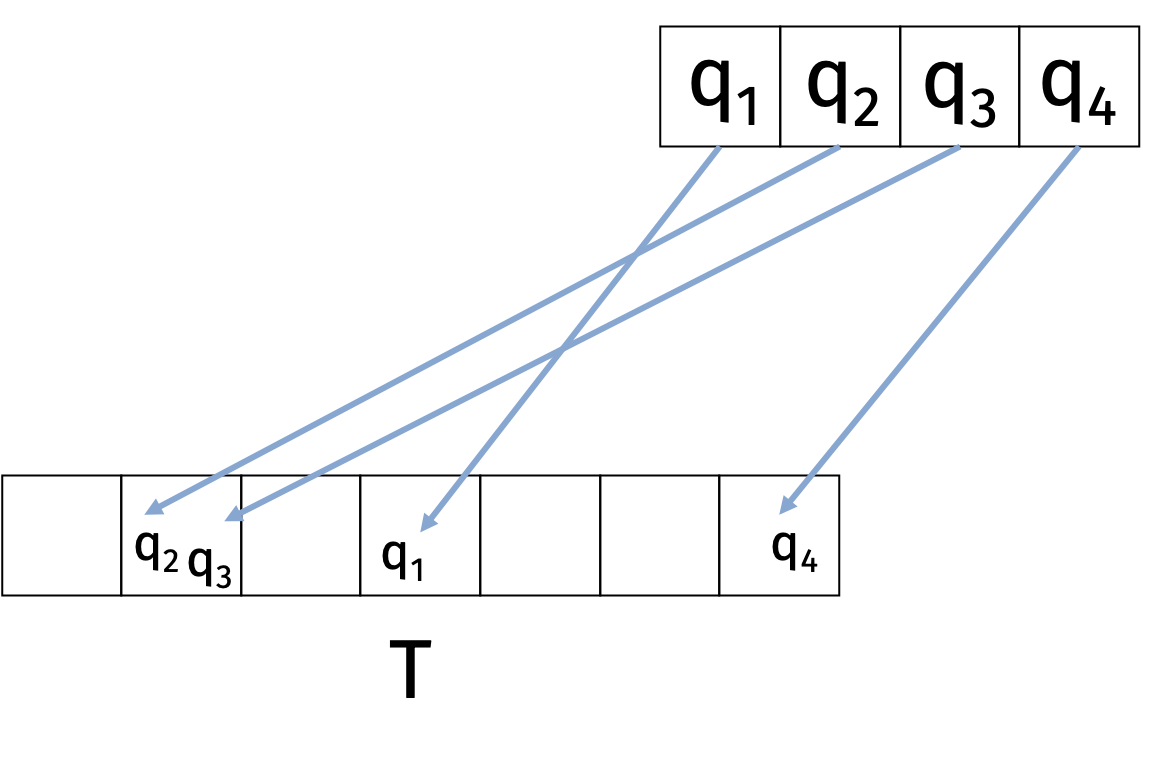
\includegraphics[width=.8\textwidth]{basicScheme.png}
	\end{center}
\end{frame}

\begin{frame}
	\frametitle{near neighbor search}
	\textbf{Two main considerations:}
	\begin{itemize}
		\item \textbf{False Negative Rate}: What's the probability we do not find a vector that \emph{is close} to $\bv{y}$?
		\item \textbf{False Positive Rate}: What's the probability that a vector in $T(h(\bv{y}))$ \emph{is not close} to $\bv{y}$?
	\end{itemize}

A higher false negative rate means we miss near neighbors.

A higher false positive rate means increased runtime -- we need to compute $S(\bv{q},\bv{y})$ for every $\bv{q}\in T(h(\bv{y}))$ to check if it's actually close to $\bv{y}$.

\textbf{Note:} The meaning of ``close'' and ``not close'' is application dependent. E.g. we might specify that we want to find anything with Jaccard similarity $> .4$, but not with Jaccard similarity $< .2$. 
\end{frame}

\begin{frame}[t]
	\frametitle{reducing false negative rate}	
	Let's use Jaccard similarity as a running example. We will discuss LSH for inner product/Euclidean distance as well. \\

	Suppose the nearest database point $\bv{q}$ has $J(\bv{y},\bv{q}) = .4$.
	\begin{center}
	\textbf{\alert{What's the probability we do not find $\bv{q}$?}}
	\end{center}
\end{frame}

\begin{frame}
	\frametitle{reducing false negative rate}
	\begin{center}
		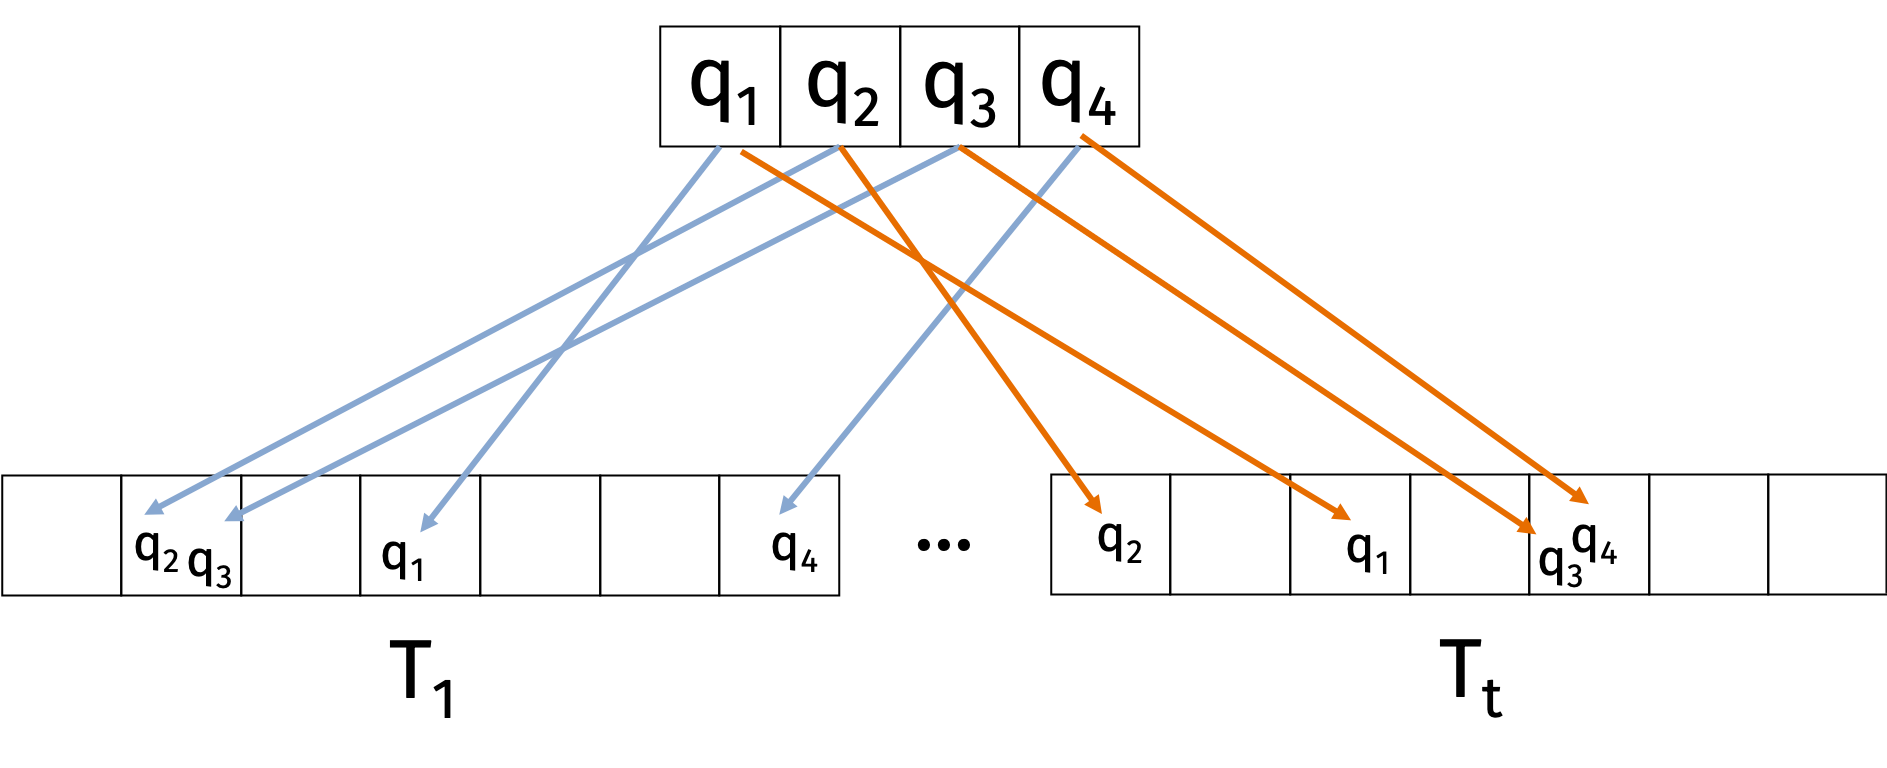
\includegraphics[width=.8\textwidth]{many_tables.png}
	\end{center}
	\textbf{Pre-processing:}
	\begin{itemize}
		\item Select $t$ independent LSH's $h_1, \ldots, h_t: \{0,1\}^d \rightarrow 1,\ldots, m$.
		\item Create tables $T_1, \ldots, T_t$, each with $m$ slots. 
		\item For $i = 1,\ldots, n$, $j = 1,\ldots, t$, 
		\begin{itemize}
			\item Insert $\bv{q}_i$ into $T_j(h_j(\bv{q}_i))$.
		\end{itemize}
	\end{itemize}
\end{frame}

\begin{frame}[t]
	\frametitle{reducing false negative rate}
	\textbf{Query:}
	\begin{itemize}
		\item Want to find near neighbors of input $\bv{y}\in\{0,1\}^d$.
		\item Linear scan through all vectors in $T_1(h_1(\bv{y}))\cup T_2(h_2(\bv{y}))\cup \ldots, T_t(h_t(\bv{y}))$.
	\end{itemize}

\vspace{2em}
	Suppose the nearest database point $\bv{q}$ has $J(\bv{y},\bv{q}) = .4$.
	\begin{center}
		\textbf{\alert{What's the probability we find $\bv{q}$?}}
	\end{center}
	
	\vskip0pt plus 1filll
	\hspace{-1em}\scriptsize($10$, $99\%$)
\end{frame}

\begin{frame}[t]
	\frametitle{what happens to false positives?}
	Suppose there is some other database point $\bv{z}$ with $J(\bv{y},\bv{z}) = .2$. 
	
	What is the probability we will need to compute $J(\bv{z},\bv{y})$ in our hashing scheme with one table? I.e. the probability that $\bv{y}$ hashes into at least one bucket containing $\bv{z}$. 
	
	\vspace{4em}
	{\textbf{\alert{In the new scheme with $t=10$ tables?}}}
	
	\vskip0pt plus 1filll
	\hspace{-1em}\scriptsize($89\%$)
\end{frame}

\begin{frame}[t]
	\frametitle{reducing false positives}
	\small
	\vspace{-.5em}
	\begin{center}
	\textbf{Change our locality sensitive hash function}.
	\vspace{-.5em}
	\end{center}
	\emph{Tunable} LSH for Jaccard similarity:
	\vspace{-.5em}
	\begin{itemize}
		\item Choose parameter $r \in \mathbb{Z}^+$.
		\item Let $c_1, \ldots, c_r: \{0,1\}^d \rightarrow [0,1]$ be independnt random MinHash's.
		\item Let $g: [0,1]^r \rightarrow \{1, \ldots, m\}$ be a uniform random hash function.
		\item Let $h(\bv{x}) = g(c_1(\bv{x}), \ldots, c_r(\bv{x})).$
	\end{itemize}
\vspace{-1em}
	\begin{center}
			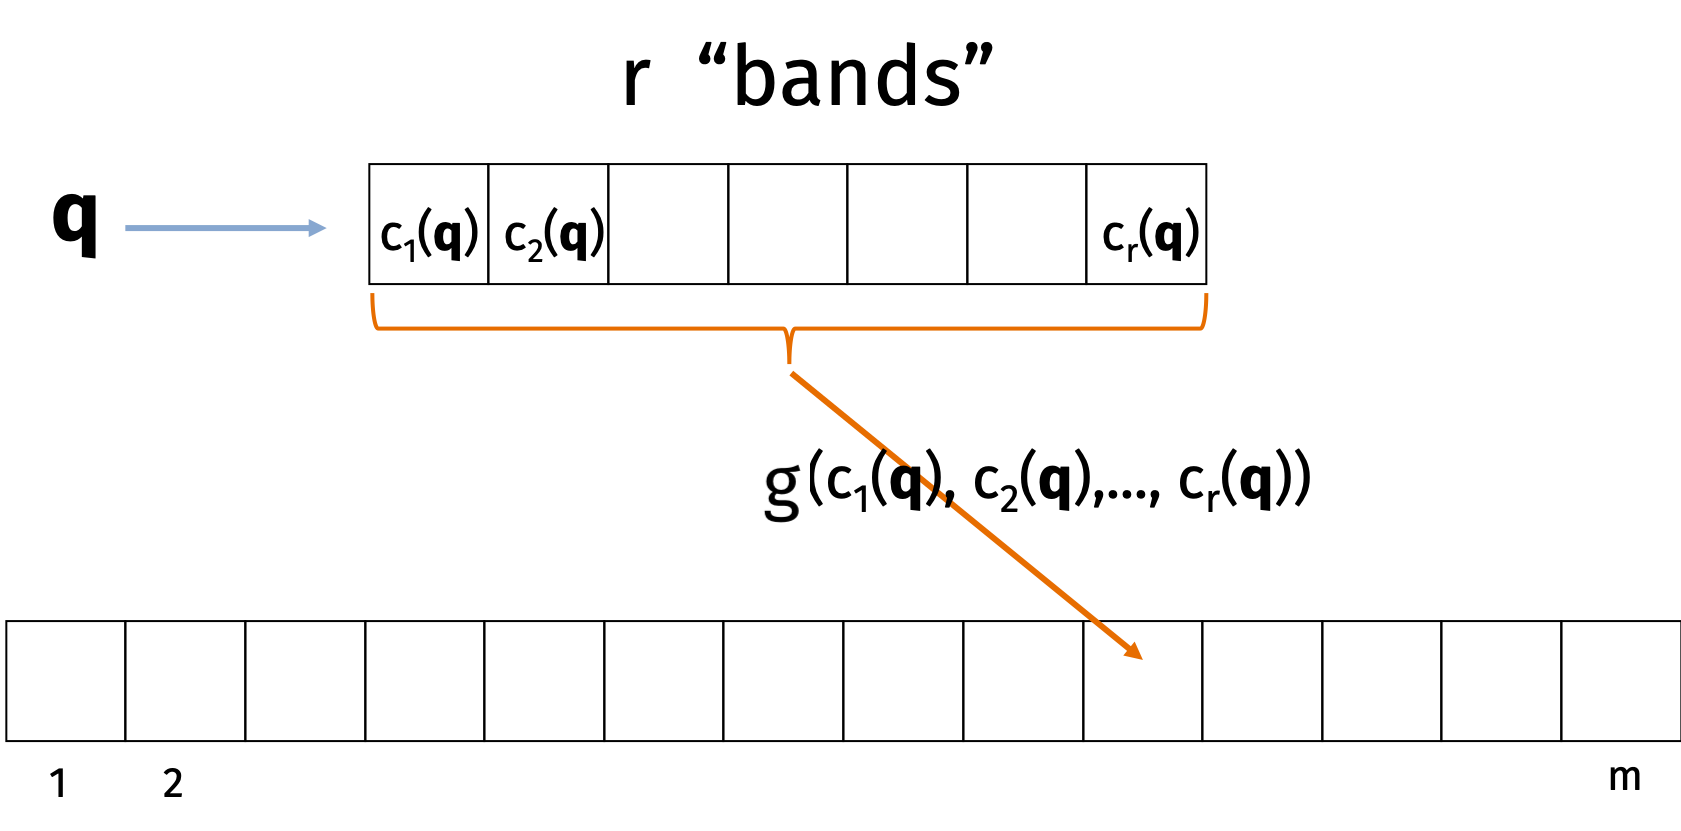
\includegraphics[width=.8\textwidth]{banded_hash.png}
	\end{center}


\end{frame}

\begin{frame}[t]
	\frametitle{reducing false positives}
	\small
	\emph{Tunable} LSH for Jaccard similarity:
	\begin{itemize}
		\item Choose parameter $r \in \mathbb{Z}^+$.
		\item Let $c_1, \ldots, c_r: \{0,1\}^d \rightarrow [0,1]$ be random MinHash.
		\item Let $g: [0,1]^r \rightarrow \{1, \ldots, m\}$ be a uniform random hash function.
		\item Let $h(\bv{x}) = g(c_1(\bv{x}), \ldots, c_r(\bv{x})).$
	\end{itemize}
	
	If $J(\bv{q},\bv{y}) = v$, then $\Pr\left[h(\bv{q}) == h(\bv{y})\right] = $
	
\end{frame}

\begin{frame}[t]
	\frametitle{tunable lsh}
	\begin{center}
		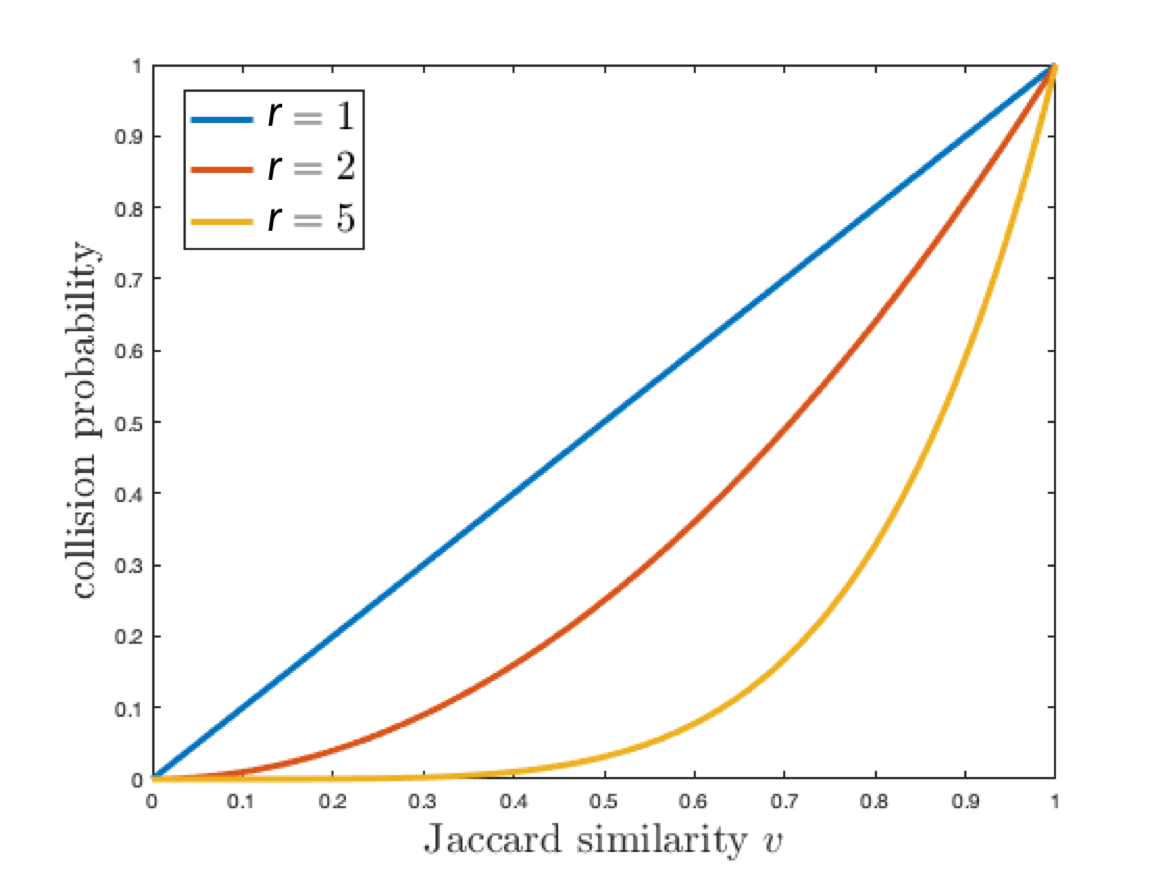
\includegraphics[width=.8\textwidth]{tuning_minhash.png}
	\end{center}
\end{frame}

\begin{frame}[t]
	\frametitle{tunable lsh}
	Full LSH cheme has two parameters to tune:
	\begin{center}
		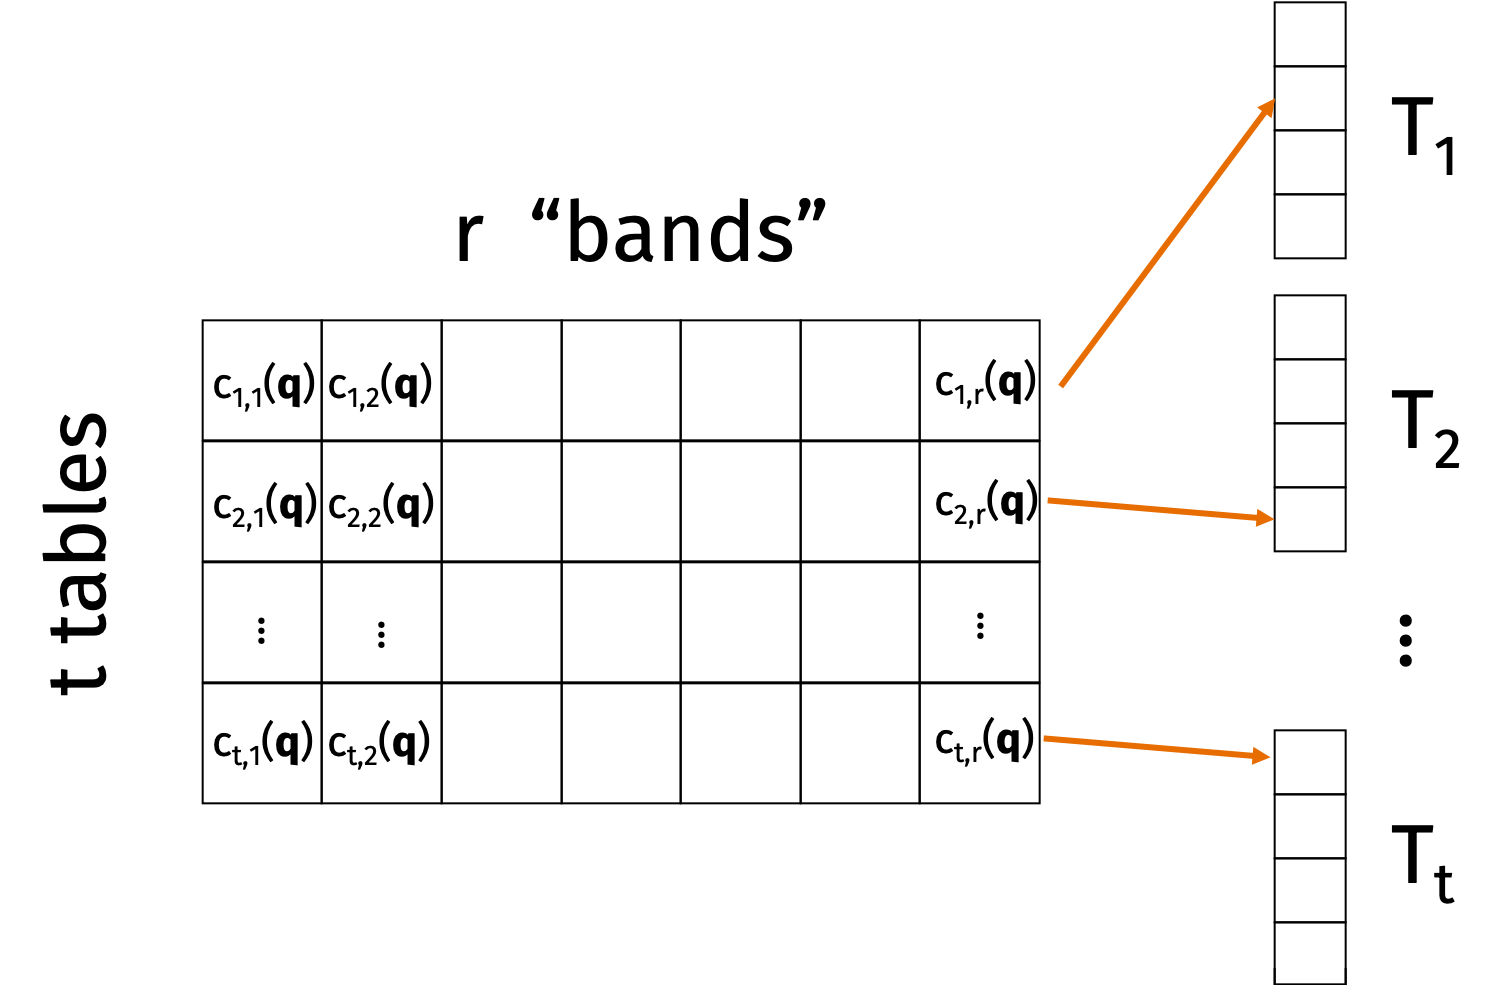
\includegraphics[width=.8\textwidth]{full_scheme.png}
	\end{center}
\end{frame}

\begin{frame}[t]
	\frametitle{tunable lsh}
	Effect of \textbf{increasing number of tables} $t$ on:
	\begin{center}
		False Negatives \hspace{6em} False Positives
	\end{center}
\vspace{4em}
	Effect of \textbf{increasing number of bands} $r$ on:
\begin{center}
	False Negatives \hspace{6em} False Positives
\end{center}
\end{frame}

%\begin{frame}
%	\frametitle{some examples}
%	Choose tables $t$ large enough so false negative rate to $1\%$.
%	\begin{center}
%		\alert{\textbf{Parameter:} $\mathbf{r = 1}$.}
%	\end{center}
%	Chance we find $\bv{q}$ with $J(\bv{y},\bv{q}) = .8$:
%	\vspace{5em}
%	
%	Chance we need to check $\bv{z}$ with $J(\bv{y},\bv{z}) = .4$:
%\end{frame}
%
%\begin{frame}
%	\frametitle{some examples}
%	Choose tables $t$ large enough so false negative rate to $1\%$.
%	\begin{center}
%		\alert{\textbf{Parameter:} $\mathbf{r = 2}$.}
%	\end{center}
%	Chance we find $\bv{q}$ with $J(\bv{y},\bv{q}) = .8$:
%	\vspace{5em}
%	
%	Chance we need to check $\bv{z}$ with $J(\bv{y},\bv{z}) = .4$:
%\end{frame}
%
%\begin{frame}
%	\frametitle{some examples}
%	Choose tables $t$ large enough so false negative rate to $1\%$.
%	\begin{center}
%		\alert{\textbf{Parameter:} $\mathbf{r = 5}$.}
%	\end{center}
%	Chance we find $\bv{q}$ with $J(\bv{y},\bv{q}) = .8$:
%	\vspace{5em}
%	
%	Chance we need to check $\bv{z}$ with $J(\bv{y},\bv{z}) = .4$:
%\end{frame}

\begin{frame}
	\frametitle{$s$-curve tuning}
	Probability we check $\bv{q}$ when querying $\bv{y}$ if $J(\bv{q},\bv{y}) = v$:
	\begin{align*}
%	\approx 	1 - (1 - v^r)^t
	\end{align*}
	\begin{center}
		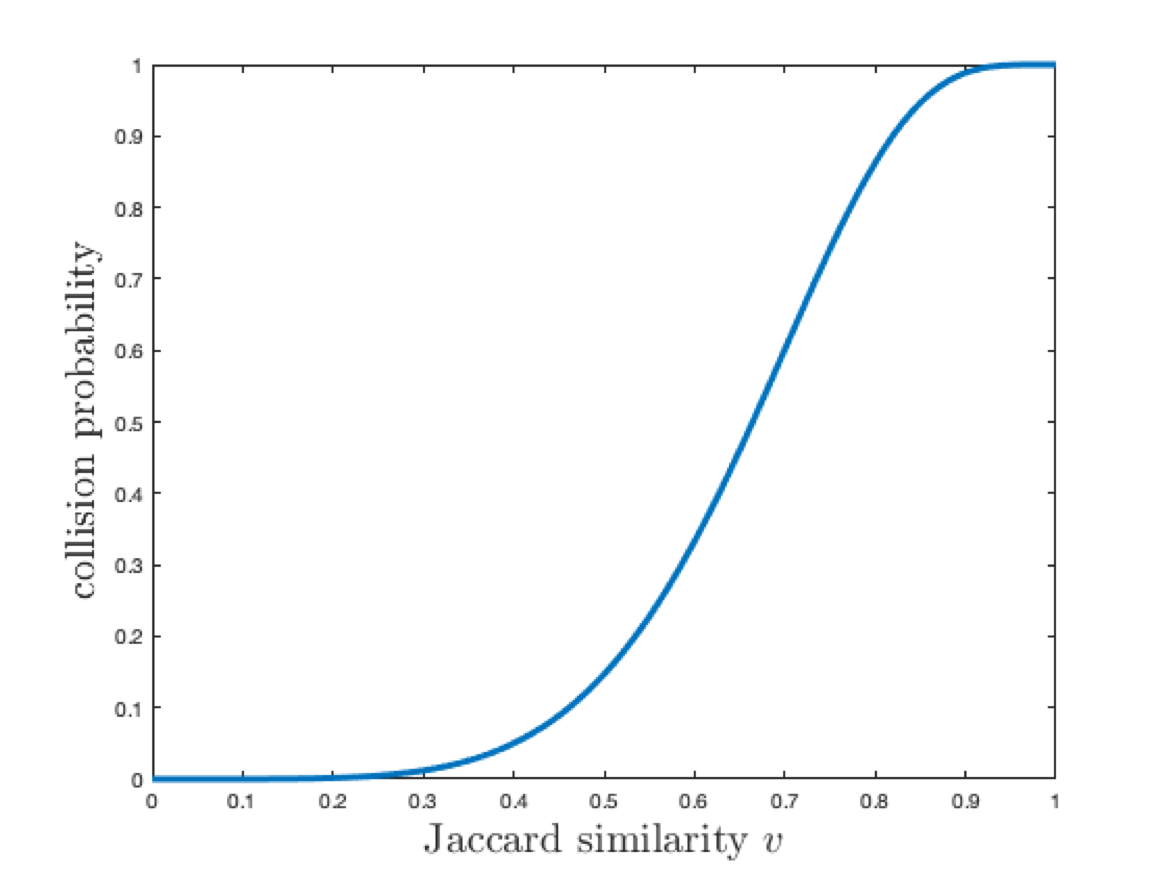
\includegraphics[width=.6\textwidth]{scurve_5_5.png}
		
		$r = 5, t = 5$
	\end{center}
\end{frame}

\begin{frame}
	\frametitle{$s$-curve tuning}
	Probability we check $\bv{q}$ when querying $\bv{y}$ if $J(\bv{q},\bv{y}) = v$:
	\begin{align*}
	\approx 1 - (1 - v^r)^t
	\end{align*}
	\begin{center}
		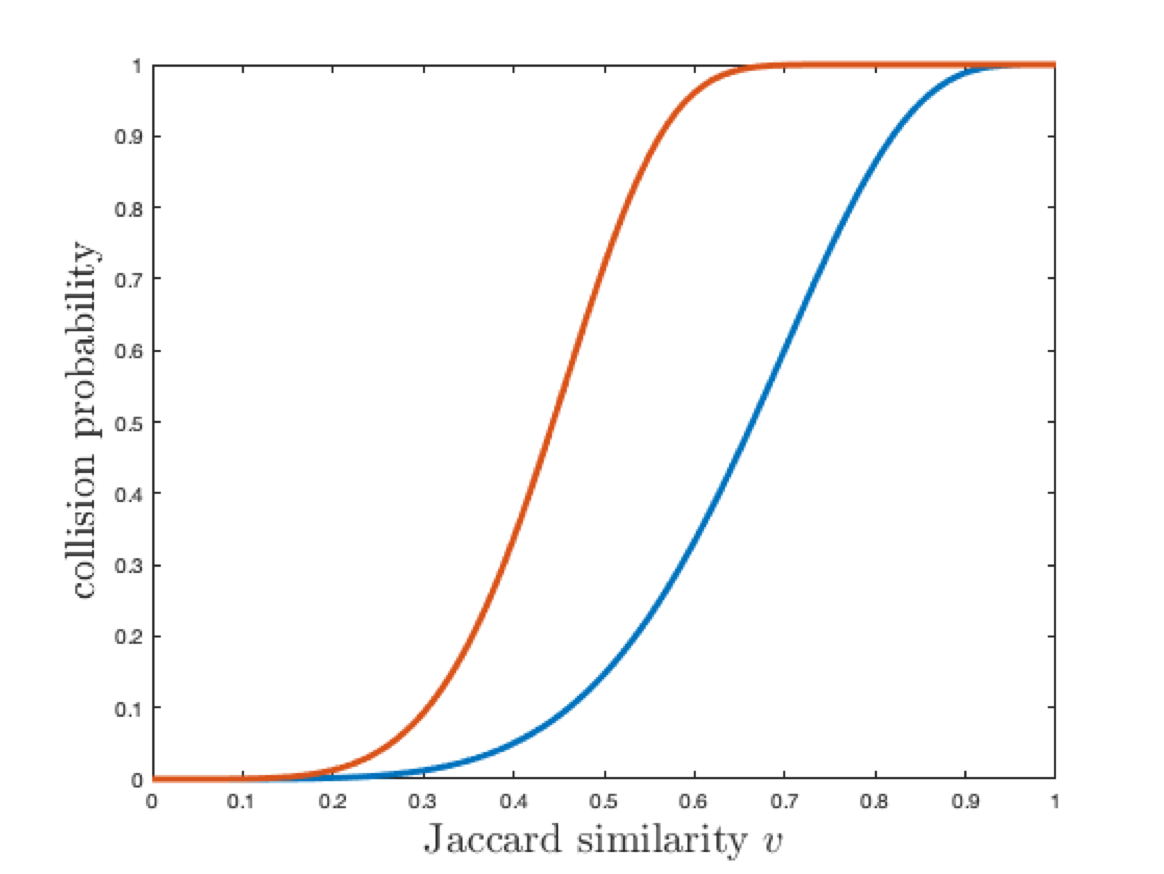
\includegraphics[width=.6\textwidth]{scurve_5_40.png}
		
		$r = 5, t = 40$
	\end{center}
\end{frame}

\begin{frame}
	\frametitle{$s$-curve tuning}
	Probability we check $\bv{q}$ when querying $\bv{y}$ if $J(\bv{q},\bv{y}) = v$:
	\begin{align*}
	\approx 1 - (1 - v^r)^t 
	\end{align*}
	\begin{center}
		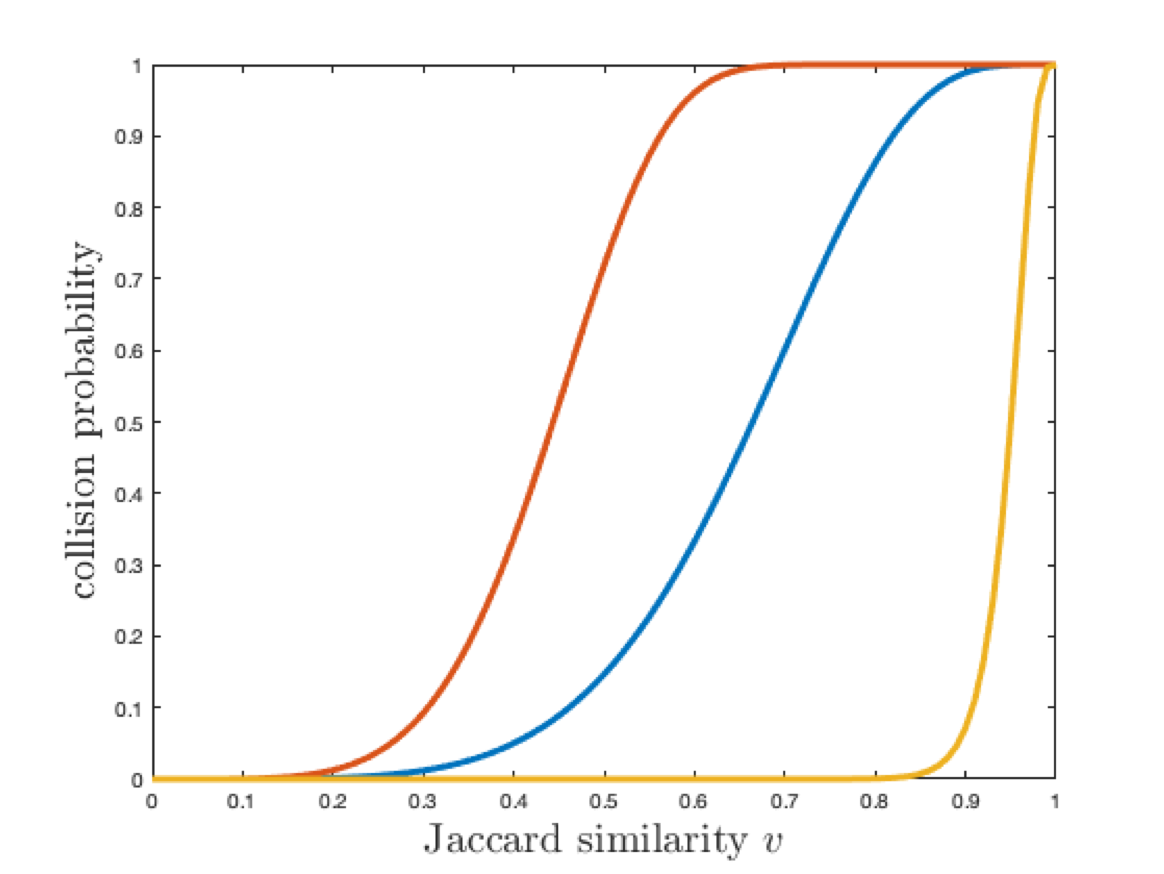
\includegraphics[width=.6\textwidth]{scurve_40_5.png}
		
		$r = 40, t = 5$
	\end{center}
\end{frame}

\begin{frame}
	\frametitle{$s$-curve tuning}
	Probability we check $\bv{q}$ when querying $\bv{y}$ if $J(\bv{q},\bv{y}) = v$:
	\begin{align*}
	1 - (1 - v^r)^t
	\end{align*}
	\begin{center}
		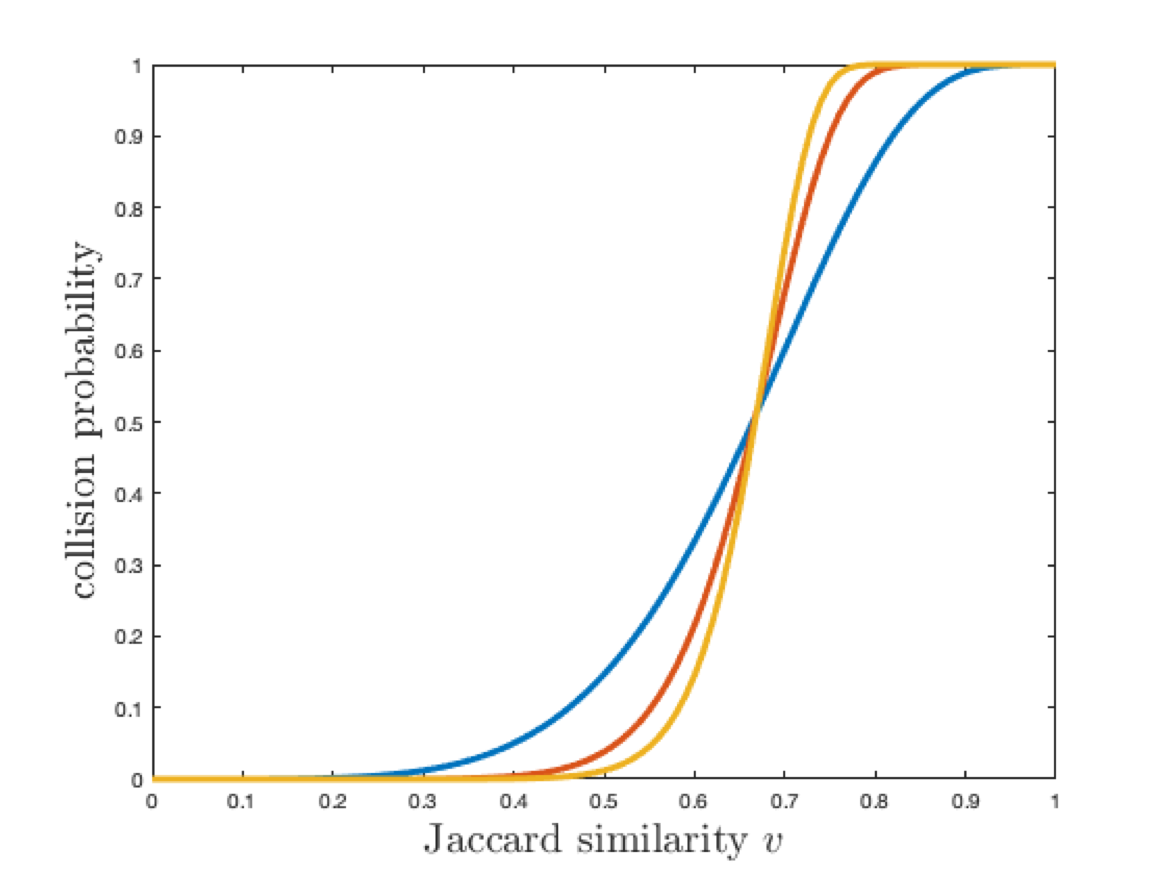
\includegraphics[width=.6\textwidth]{scurve_centered.png}
		
		Increasing both $r$ and $t$ gives a steeper curve. 
		
		\alert{\textbf{Better for search, but worse space complexity}.}
	\end{center}
\end{frame}

\begin{frame}
	\frametitle{fixed threshold}
	\small
	\textbf{Use Case 1:} Fixed threshold.
	\begin{itemize}
		\item Shazam wants to find match to audio clip $\bv{y}$ in a database of 10 million  clips.
		\item There are 10 \emph{true matches} with $J(\bv{y},\bv{q}) > .9$.
		\item There are 10,000 \emph{near matches} with $J(\bv{y},\bv{q}) \in [.7,.9]$.
		\item All other items have $J(\bv{y},\bv{q}) < .7$.
	\end{itemize}
	With $r = 25$ and $t = 40$, 
	\begin{itemize}
		\item Hit probability for $J(\bv{y},\bv{q}) > .9$ is $\gtrsim 1 - (1 - .9^{25})^{40} = .95$
		\item Hit probability for $J(\bv{y},\bv{q}) \in [.7,.9]$ is $\lesssim 1 - (1 - .9^{25})^{40} = .95$
		\item Hit probability for $J(\bv{y},\bv{q}) < .7$ is $\lesssim 1 - (1 - .7^{25})^{40} = .005$
	\end{itemize}
	\textbf{Upper bound on total number of items checked:} 
	\begin{align*}
	10 + .95 \cdot 10,000 + .005 \cdot 9,989,990 \alert{\approx 60,000 \ll 10,000,000}.
	\end{align*}  
\end{frame}

\begin{frame}
	\frametitle{fixed threshold}
	\begin{center}
	Space complexity: 40 hash tables \alert{$\approx 40\cdot O(n)$}. 
	
	\textbf{Directly trade space for fast search.}
	\end{center}
\end{frame}

\begin{frame}
	\frametitle{lsh based nearest-neighbor in theory}
	Possible to prove concrete worst-case results for distance functions that satisfy triangle inequality. 
	\begin{theorem}[Indyk, Motwani, 1998. Point Location in Ball]
		Fix a distance $R$. If there exists some $q$ with $\|\bv{q} - \bv{y}\|_0 \leq R$, return a vector $\tilde{\bv{q}}$ with $\|\tilde{\bv{q}} - \bv{y}\|_0 \leq C\cdot R$ in:
		\begin{itemize}
			\item Time: $O\left(n^{1/C}\right)$.
			\item Space: $O\left(n^{1 + 1/C} + nd\right)$. 
		\end{itemize}
	\end{theorem}
	$\|\bv{q} - \bv{y}\|_0 = $ ``hamming distance" = number of elements that differ between $\bv{q}$ and $\bv{y}$. 

	\begin{center}
	\textbf{\alert{If there is no point at distance $R$, algorithm does not need to return anything.}}
	\end{center}
\end{frame}

\begin{frame}
	\frametitle{lsh based nearest-neighbor in theory}
	To obtain a nearest-neighbor search algorithm build multiple data structures for exponentially growing distances:
	\begin{align*}
	&R & &2 R & &4R & &8R & \ldots 
	\end{align*}
	Search from most accurate level to least accurate. 

	\begin{center}
	\only<1>{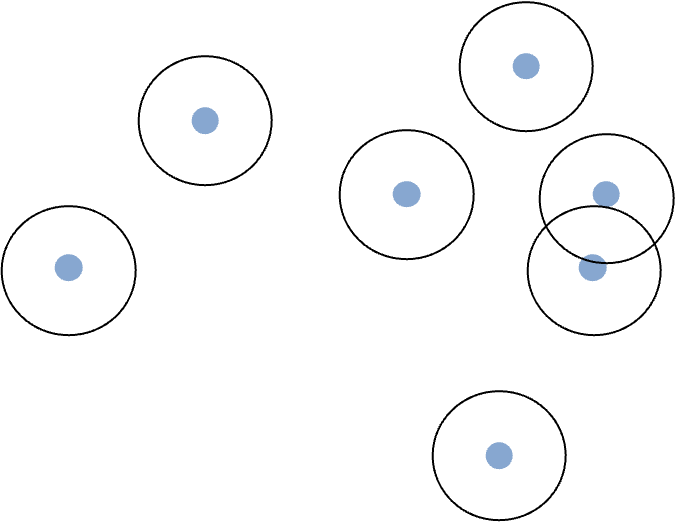
\includegraphics[width = .5\textwidth]{pleb1.png}}
	\only<2>{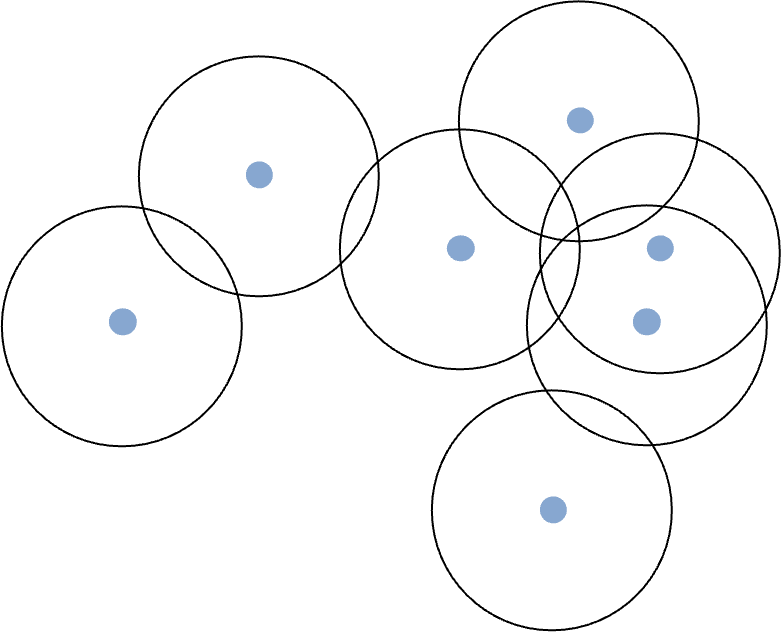
\includegraphics[width = .5\textwidth]{pleb2.png}}
	\only<3>{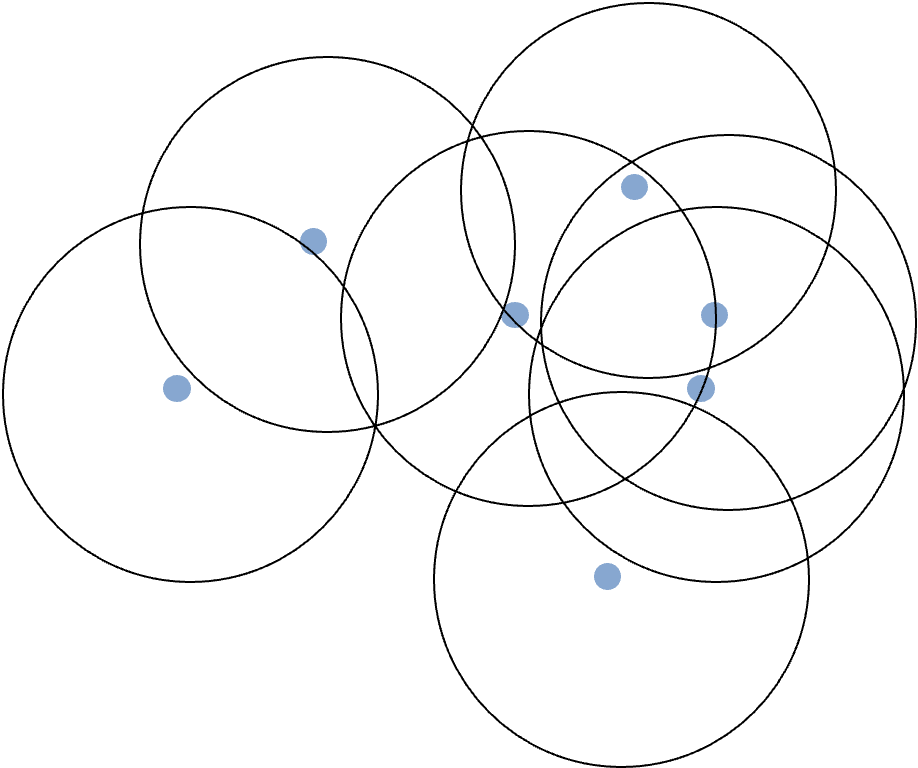
\includegraphics[width = .5\textwidth]{pleb3.png}}
	\end{center}
\end{frame}


\begin{frame}
	\frametitle{approximate nearest neighbor search}
	Total number of levels = $O(\log(d_{\max}/d_{\min}))$, where $d_{\max} = \max_{i,j}\|\bv{q}_i - \bv{q}_j\|$ and $d_{\min} = \min_{i,j}\|\bv{q}_i - \bv{q}_j\|$. $d_{\max}/d_{\min}$ is called the \textbf{dynamic range}.

		\begin{theorem}[Indyk, Motwani, 1998]
		Let $q$ be the closest database vector to $\bv{y}$. Return a vector $\tilde{\bv{q}}$ with $\|\tilde{\bv{q}} - \bv{y}\|_0 \leq C\cdot \|{\bv{q}} - \bv{y}\|_0$ in:
		\begin{itemize}
			\item Time: $\tilde{O}\left(n^{1/C}\right)$.
			\item Space: $\tilde{O}\left(n^{1 + 1/C} + nd\right)$. 
		\end{itemize}
	\end{theorem}
	Similar results can be proven for other metrics, including Euclidean distance. But you need a good LSH function.
\end{frame}

\begin{frame}
	\frametitle{other lsh functions}
	\begin{center}
	Good locality sensitive hash functions exists for other similarity measures.
	\end{center}
	\textbf{Cosine similarity $\cos\left(\theta(\bv{x},\bv{y})\right) = \frac{\langle \bv{x},\bv{y}\rangle}{\|\bv{x}\|_2\|\bv{y}\|_2}$:}
	\begin{center}
		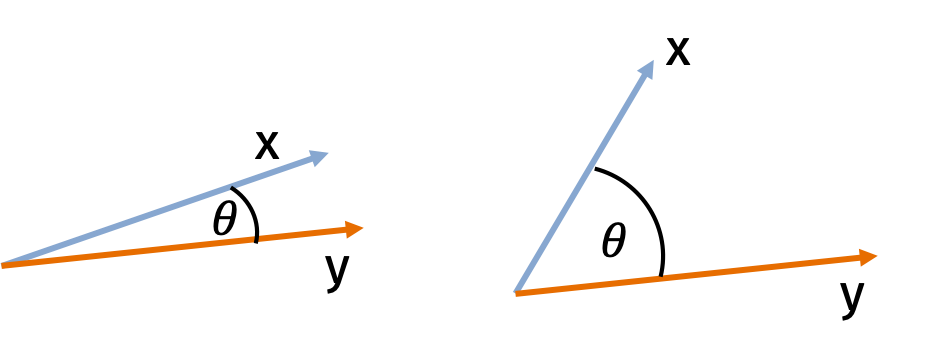
\includegraphics[width=.7\textwidth]{cos_sim.png}
		
		$-1 \leq \cos\left(\theta(\bv{x},\bv{y})\right) \leq 1$.
	\end{center}
\end{frame}

\begin{frame}
	\frametitle{cosine similarity}
		Cosine similarity is natural ``inverse" for Euclidean distance when $\|\bv{x}\|_2^2 = \|\bv{y}\|_2^2 = 1$ (often the case for ML-based embeddings).


	\vspace{5em}
	LSH functions also exist for Euclidean distance, but are a bit more complex to describe/analyze. See [Andoni, Indyk, 2006] if you are interested.
\end{frame}

\begin{frame}
	\frametitle{simhash}
	Locality sensitive hash for \textbf{cosine similarity}:
	\begin{itemize}
		\item Let $\bv{g} \in \R^d$ be randomly chosen with each entry $\mathcal{N}(0,1)$. 
		\item Let $f: \{-1,1\} \rightarrow \{1,\ldots, m\}$ be a uniformly random hash function. 
		\item $h: \R^d \rightarrow \{1,\ldots, m\}$ is definied $h(\bv{x}) = f\left(\sign(\langle \bv{g}, \bv{x} \rangle)\right)$.
	\end{itemize}
	\begin{center}
		\alert{\textbf{
				\large
				If $\cos(\theta(\bv{x},\bv{y})) = v$, what is $\Pr[h(\bv{x}) == h(\bv{y})]$?
		}}
	\end{center}
\end{frame}


%\begin{frame}
%	\frametitle{simhash}
%	\begin{center}
%		\textbf{Inspired by Johnson-Lindenstrauss sketching}
%		
%		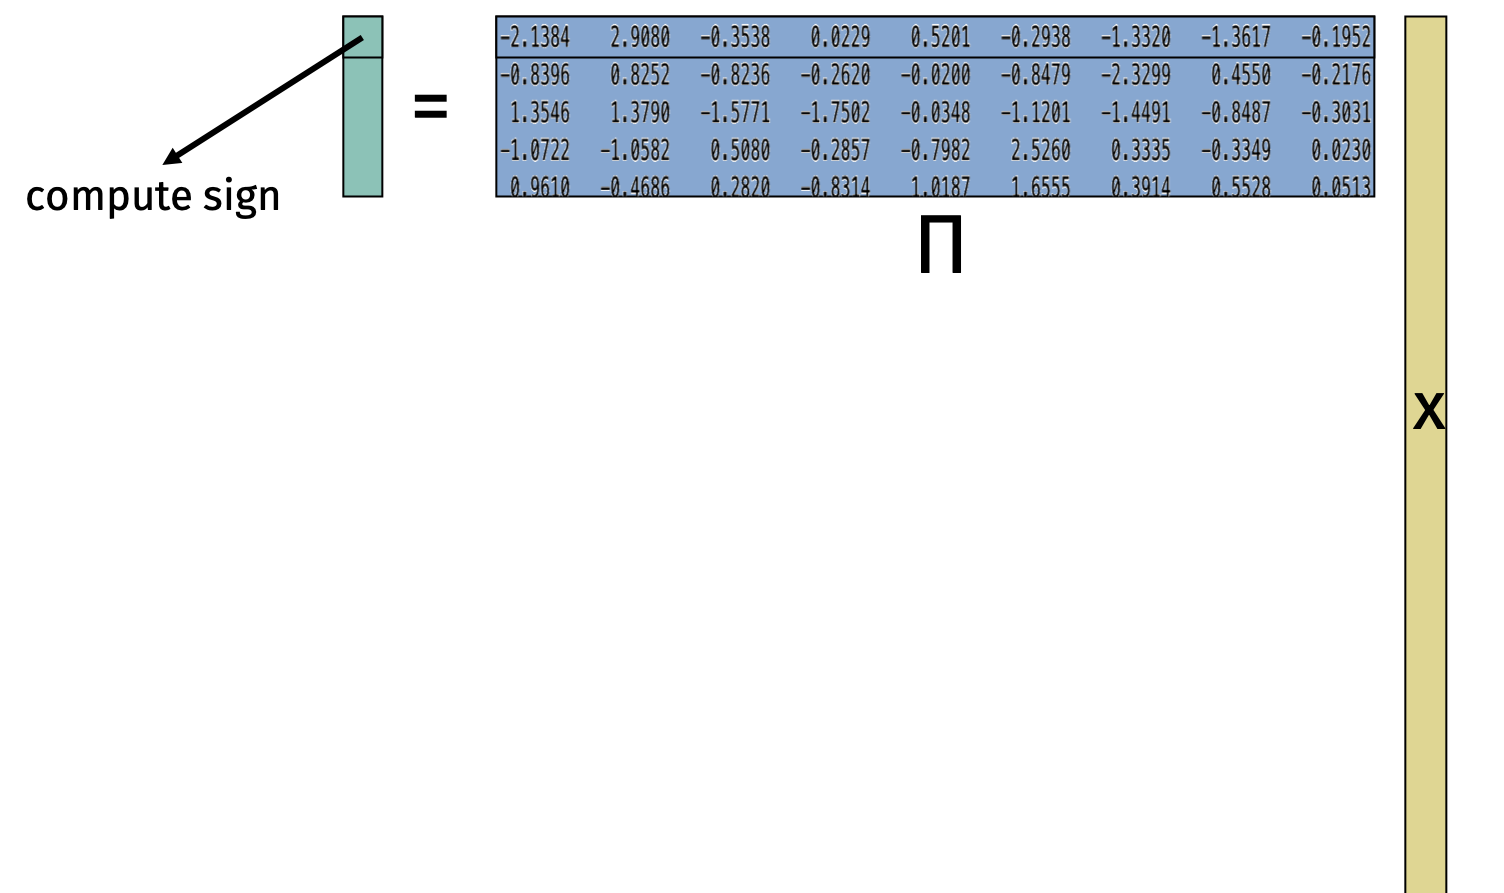
\includegraphics[width=\textwidth]{simhash_jl.png}
%	\end{center}
%\end{frame}



\begin{frame}[t]
	\frametitle{simhash analysis in 2d}
	\textbf{Theorem (to be proven):} If $\cos(\theta(\bv{x},\bv{y})) = v$, then 
	\begin{align*}
		\Pr[h(\bv{x}) == h(\bv{y})] = 1 - \frac{\theta}{\pi}  + \frac{\theta/\pi}{m}= 1 - \frac{\cos^{-1}(v)}{\pi} + \frac{\theta/\pi}{m}
	\end{align*}
	\begin{center}
		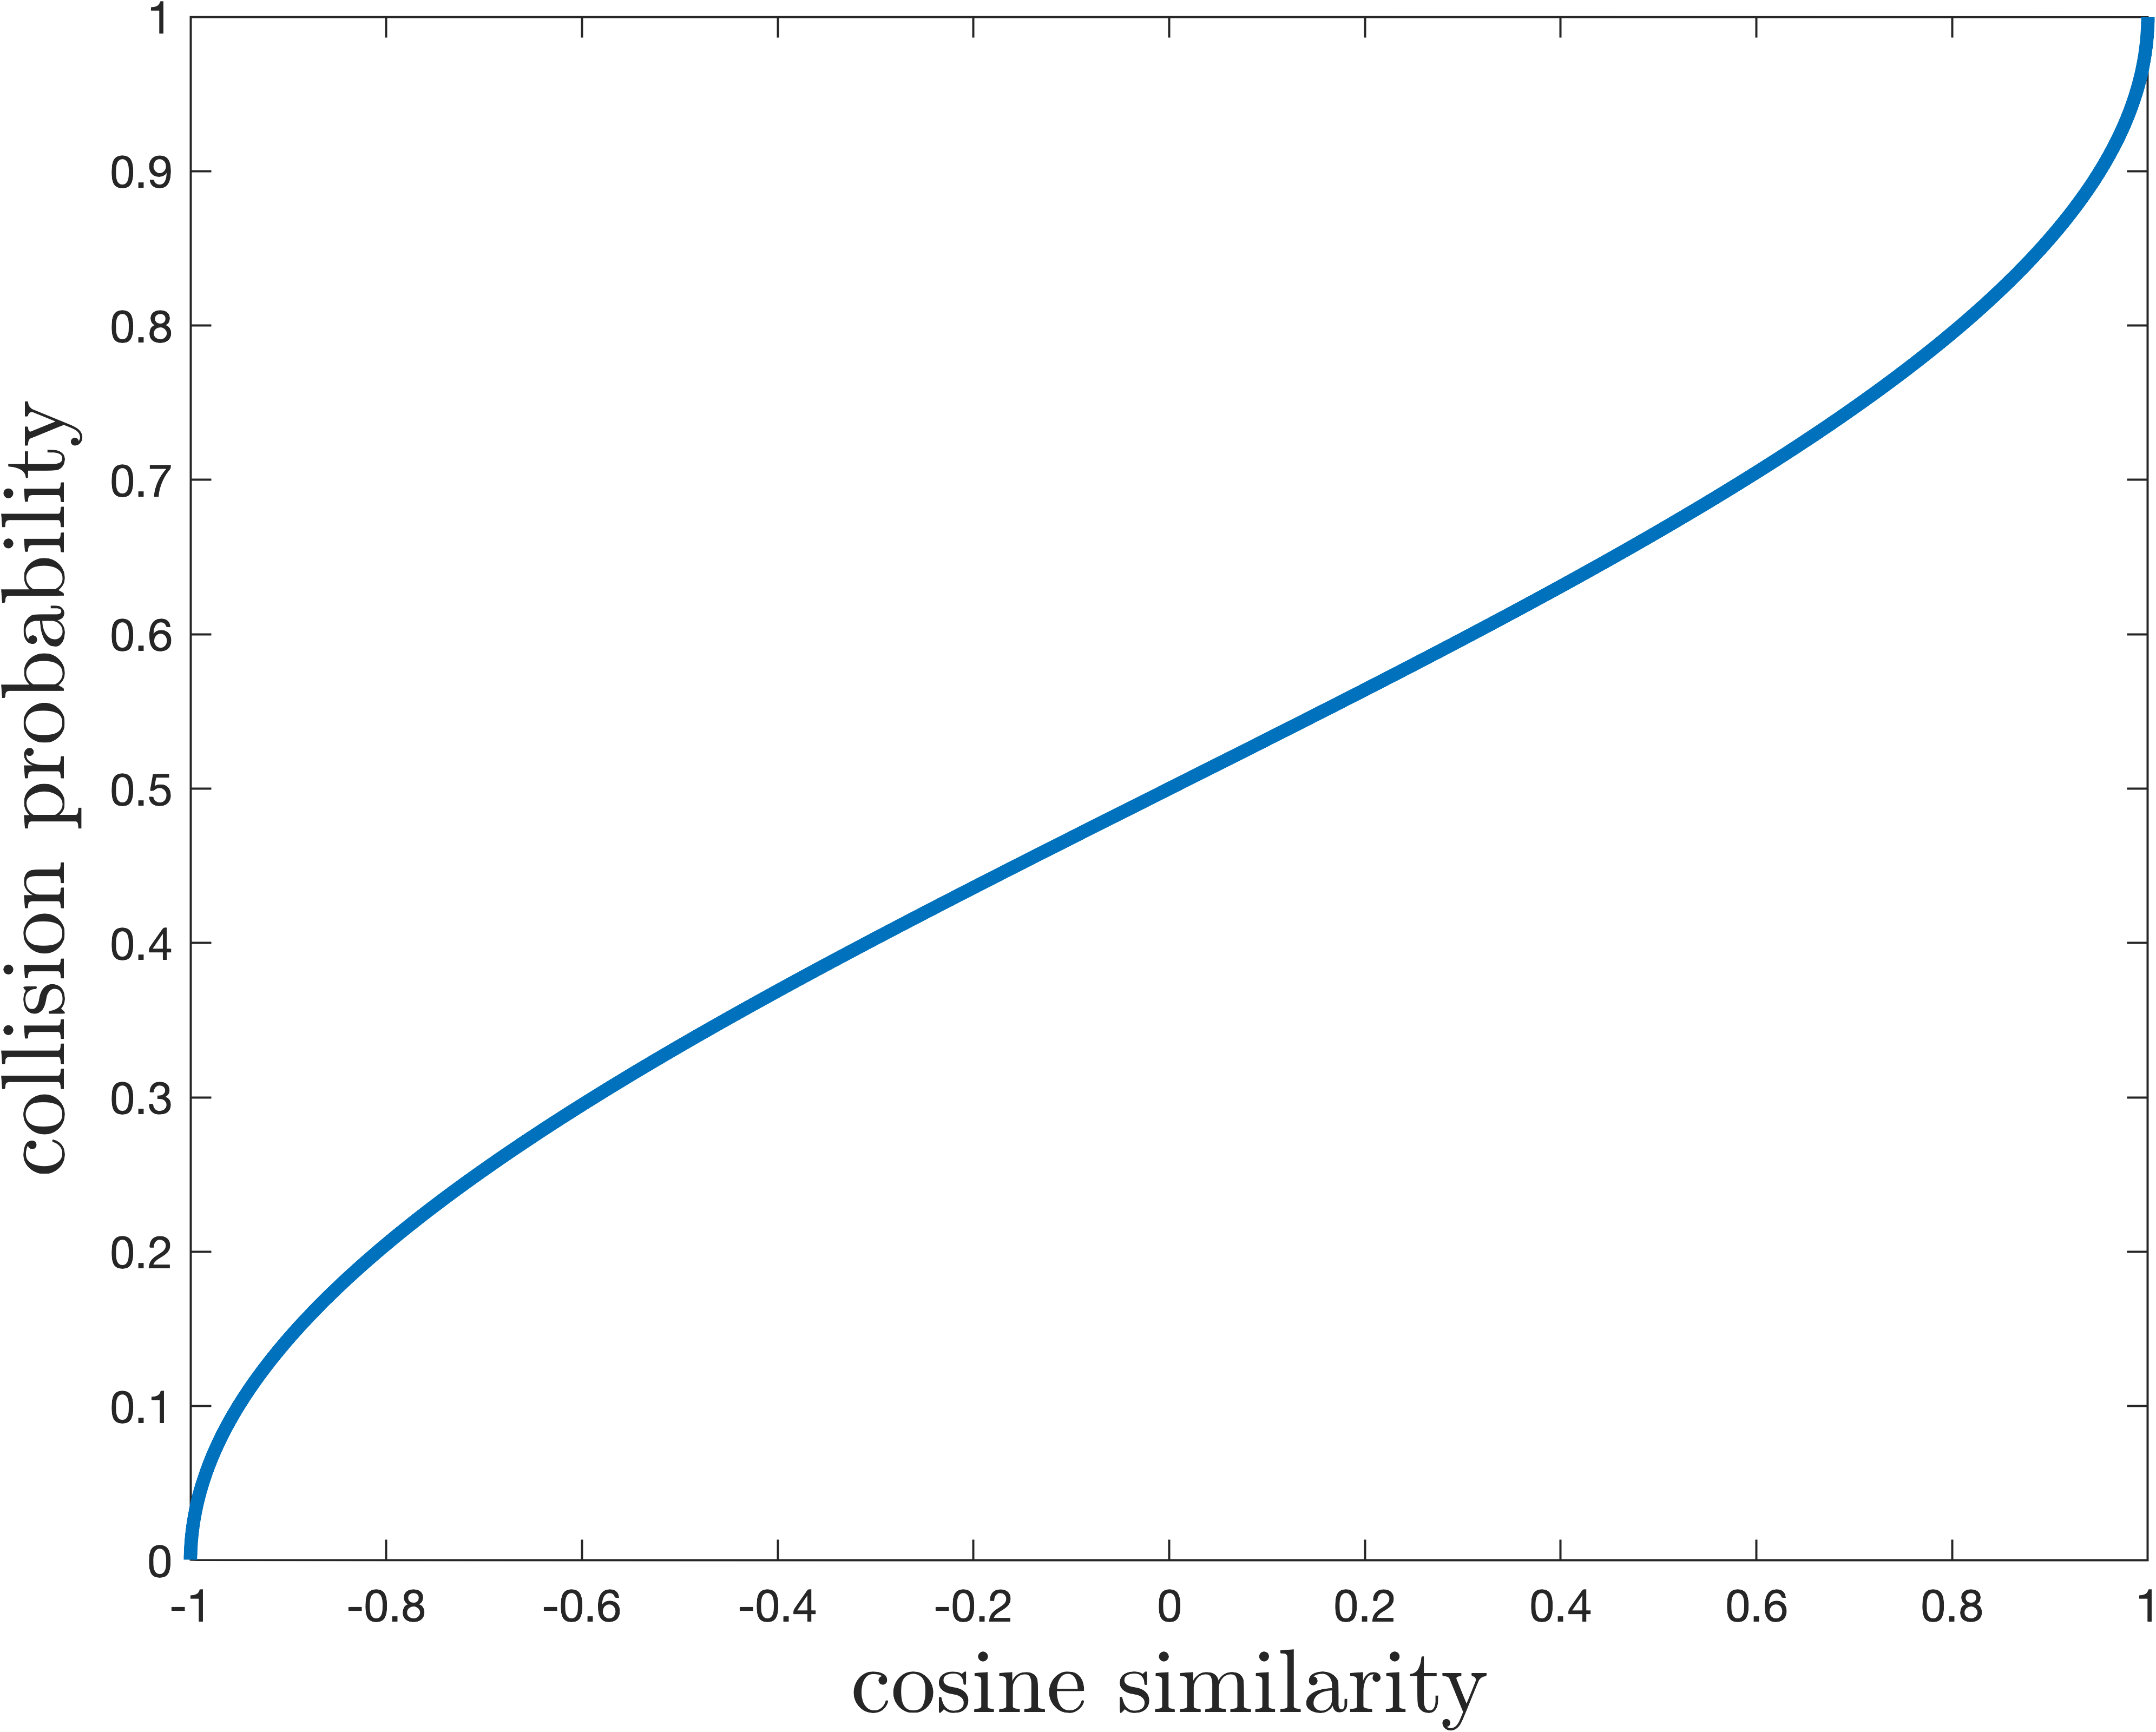
\includegraphics[width=.6\textwidth]{cosine_sim.png}
	\end{center}
\end{frame}

\begin{frame}
	\frametitle{simhash}
	SimHash can be banded, just like our MinHash based LSH function for Jaccard similarity:
	\begin{itemize}
		\item Let $\bv{g}_1,\ldots, \bv{g}_r \in \R^d$ be randomly chosen with each entry $\mathcal{N}(0,1)$. 
		\item Let $f: \{-1,1\}^r \rightarrow \{1,\ldots, m\}$ be a uniformly random hash function. 
		\item $h: \R^d \rightarrow \{1,\ldots, m\}$ is defined $h(\bv{x}) = f\left([\sign(\langle \bv{g}_1, \bv{x} \rangle),\ldots, \sign(\langle \bv{g}_r, \bv{x} \rangle)]\right)$.
	\end{itemize}
\begin{align*}
	\Pr[h(\bv{x}) == h(\bv{y})] \approx \left(1-\frac{\theta}{\pi}\right)^r
\end{align*}
\end{frame}

\begin{frame}
	\textbf{To prove:}  $\Pr[h(\bv{x}) == h(\bv{y})] \approx 1 - \frac{\theta}{\pi}$,  where $h(\bv{x}) = f\left(\sign(\langle \bv{g}, \bv{x} \rangle)\right)$ and $f$ is uniformly random hash function.
	\frametitle{simhash analysis in 2d}
	\vspace{-.5em}
	\begin{center}
		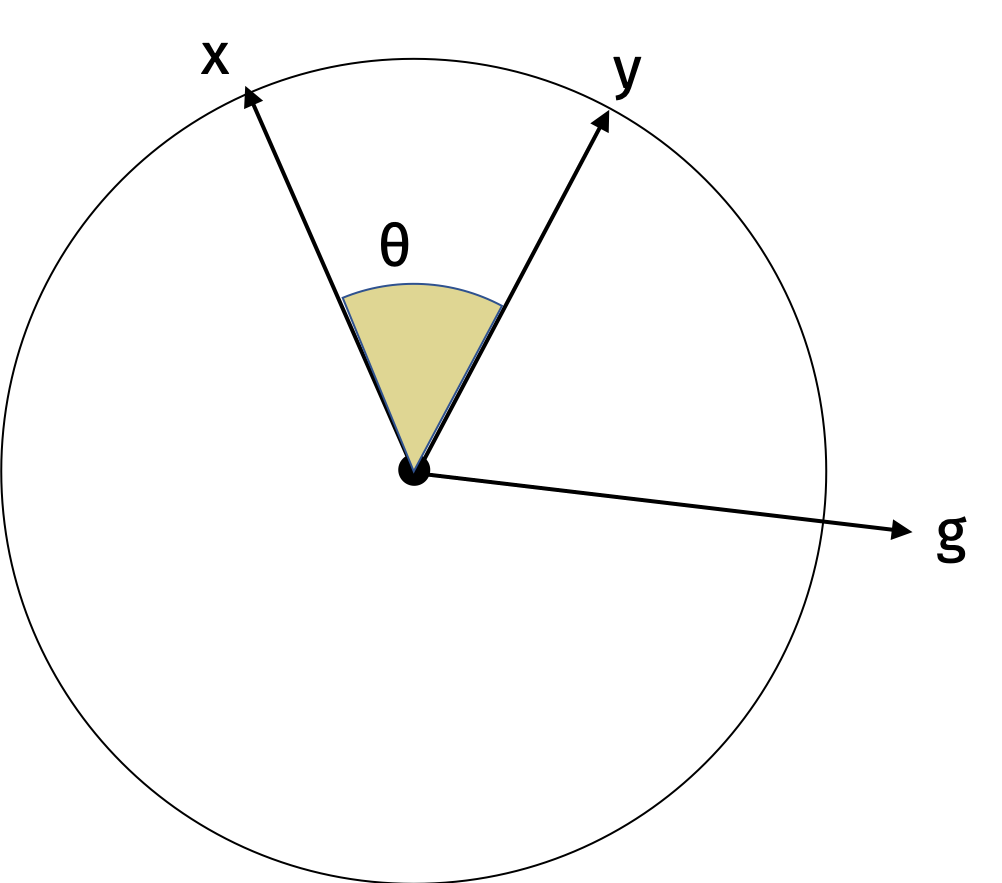
\includegraphics[width=.5\textwidth]{simhash1.png}
	\end{center}
\begin{align*}
	\Pr[h(\bv{x}) == h(\bv{y})] = z + \frac{1-z}{m} \approx z.
\end{align*}
where $z = \Pr[\sign(\langle \bv{g}, \bv{x} \rangle) == \sign(\langle \bv{g}, \bv{y} \rangle)]$
\end{frame}

\begin{frame}
	\frametitle{simhash analysis 2d}
	\vspace{-.5em}
	\begin{center}
		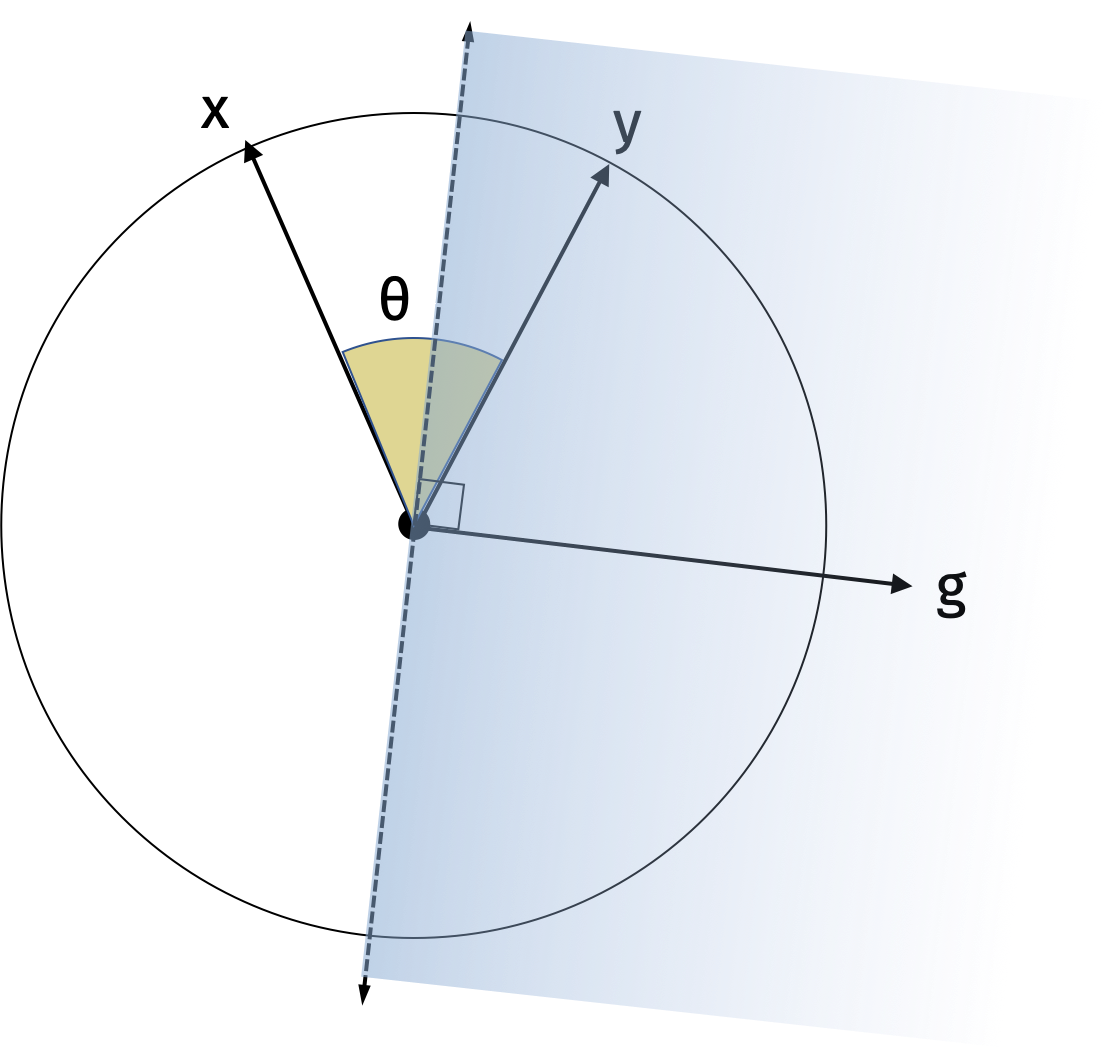
\includegraphics[width=.55\textwidth]{simhash2.png}
	\end{center}
\vspace{-.5em}
$\Pr[\sign(\langle \bv{g}, \bv{x} \rangle) == \sign(\langle \bv{g}, \bv{y} \rangle)] = $ probability $\bv{x}$ and $\bv{y}$ are on the same side of hyperplane orthogonal to $\bv{g}$.
\end{frame}

\begin{frame}
	\frametitle{simhash analysis higher dimensions}
	\begin{center}
		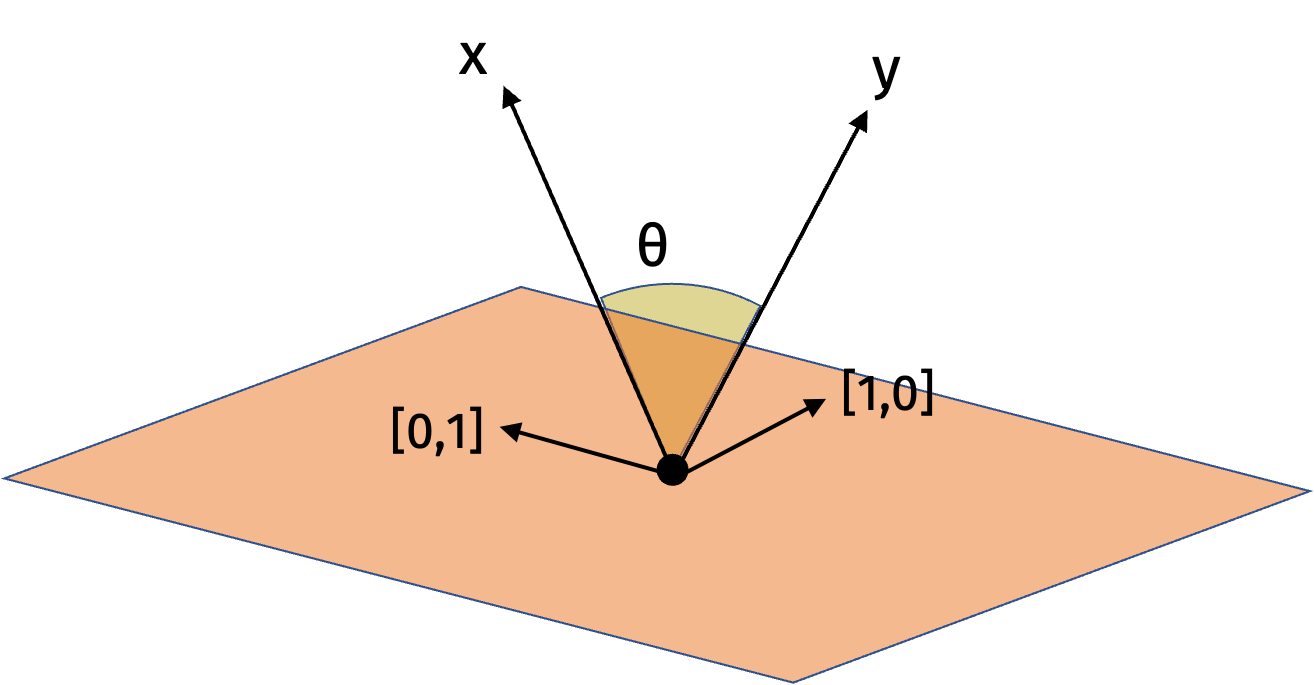
\includegraphics[width=.7\textwidth]{high_dim1.png}
	\end{center}
There is always some \emph{rotation matrix} $\bv{U}$ such that $\bv{U}\bv{x},\bv{U}\bv{y}$ are spanned by the first two-standard basis vectors and have the same cosine similarity as $\bv{x}$ and $\bv{y}$.
\end{frame}

\begin{frame}
	\frametitle{simhash analysis higher dimensions}
	\begin{center}
		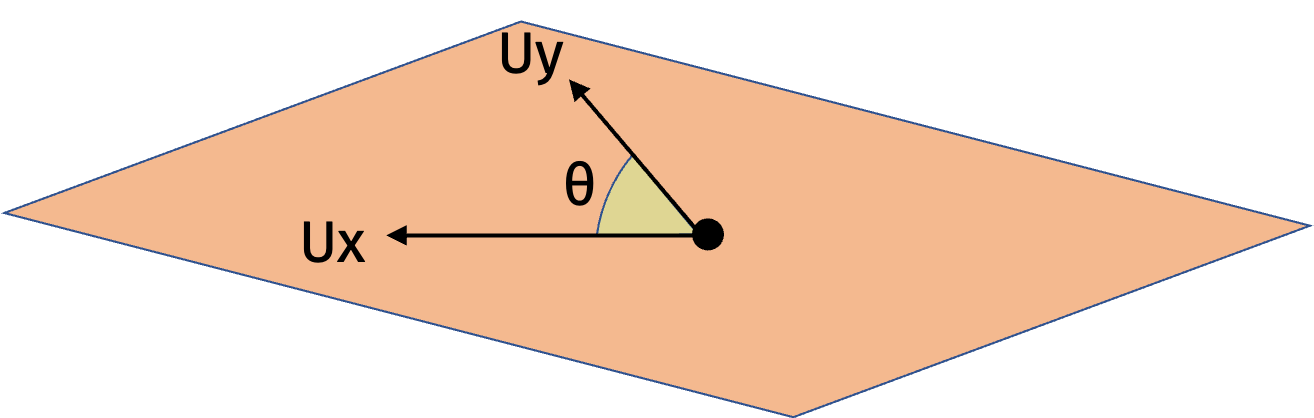
\includegraphics[width=.7\textwidth]{high_dim2.png}
	\end{center}
	There is always some \emph{rotation matrix} $\bv{U}$ such that $\bv{x},\bv{y}$ are spanned by the first two-standard basis vectors. 
	
	
	\textbf{Note:} A rotation matrix $\bv{U}$ has the property that $\bv{U}^T\bv{U} = \bv{I}$. I.e., $\bv{U}^T$ is a rotation matrix itself, which reverses the rotation of $\bv{U}$.
\end{frame}

\begin{frame}[t]
	\frametitle{simhash analysis higher dimensions}
\textbf{Claim:} 
% \begin{align*}
% 1 - \frac{\theta}{\pi} &= \Pr[\sign(\langle \bv{g}[1,2], (\bv{U}\bv{x})[1,2] \rangle) == \sign(\langle \bv{g}[1,2], (\bv{U}\bv{y}[1,2] \rangle)] \\
% &= \Pr[\sign(\langle \bv{g}, \bv{U}\bv{x} \rangle) == \sign(\langle \bv{g}, \bv{U}\bv{y} \rangle)] \\
% &\alert{= \Pr[\sign(\langle \bv{g}, \bv{x} \rangle) == \sign(\langle \bv{g}, \bv{y} \rangle)]}
% \end{align*}
\begin{align*}
	&\Pr[\sign(\langle \bv{g}, \bv{x} \rangle) == \sign(\langle \bv{g}, \bv{y} \rangle) = \Pr[\sign(\langle \bv{g}, \bv{U}\bv{x} \rangle) == \sign(\langle \bv{g}, \bv{U}\bv{y} \rangle)] \\
	&\hspace{4em}= \Pr[\sign(\langle \bv{g}[1,2], (\bv{U}\bv{x})[1,2] \rangle) == \sign(\langle \bv{g}[1,2], (\bv{U}\bv{y}[1,2] \rangle)]\\
	&\hspace{4em} = 1 - \frac{\theta}{\pi}.
	\end{align*}

	The first step is the trickiest here. Why does it hold?
\end{frame}

\begin{frame}[t]
	\frametitle{nearest-neighbor search in practice}
	LSH is widely used in practice, but is starting to get replaced by other methods. Most of these are \emph{data dependent} in some way. 

	\textbf{Starting point:} Think of LSH as a randomized \emph{space-partitioning method}.
	\begin{center}
	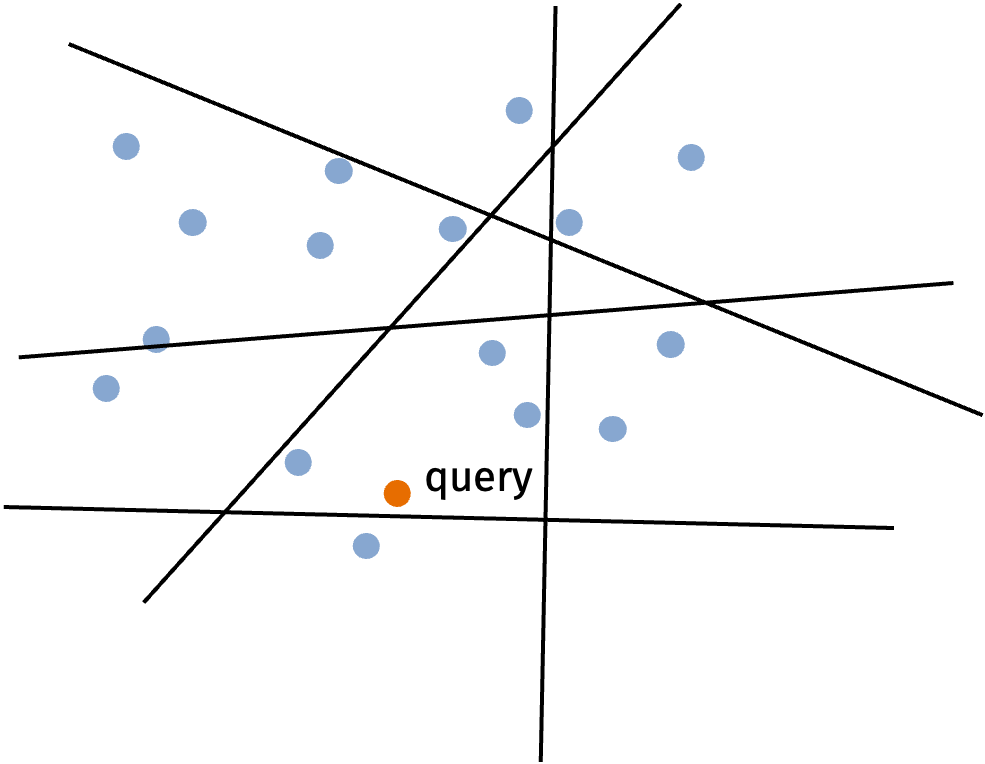
\includegraphics[width=.6\textwidth]{random_space_partition.png}
	\end{center}

\end{frame}

\begin{frame}[t]
	\frametitle{nearest-neighbor search in practice}
In practice, we can often get partitions with better \emph{margin} but partitioning in a data-dependent way. 

	\textbf{Common approach:} Split data using $k$-means clustering. 
	\begin{center}
	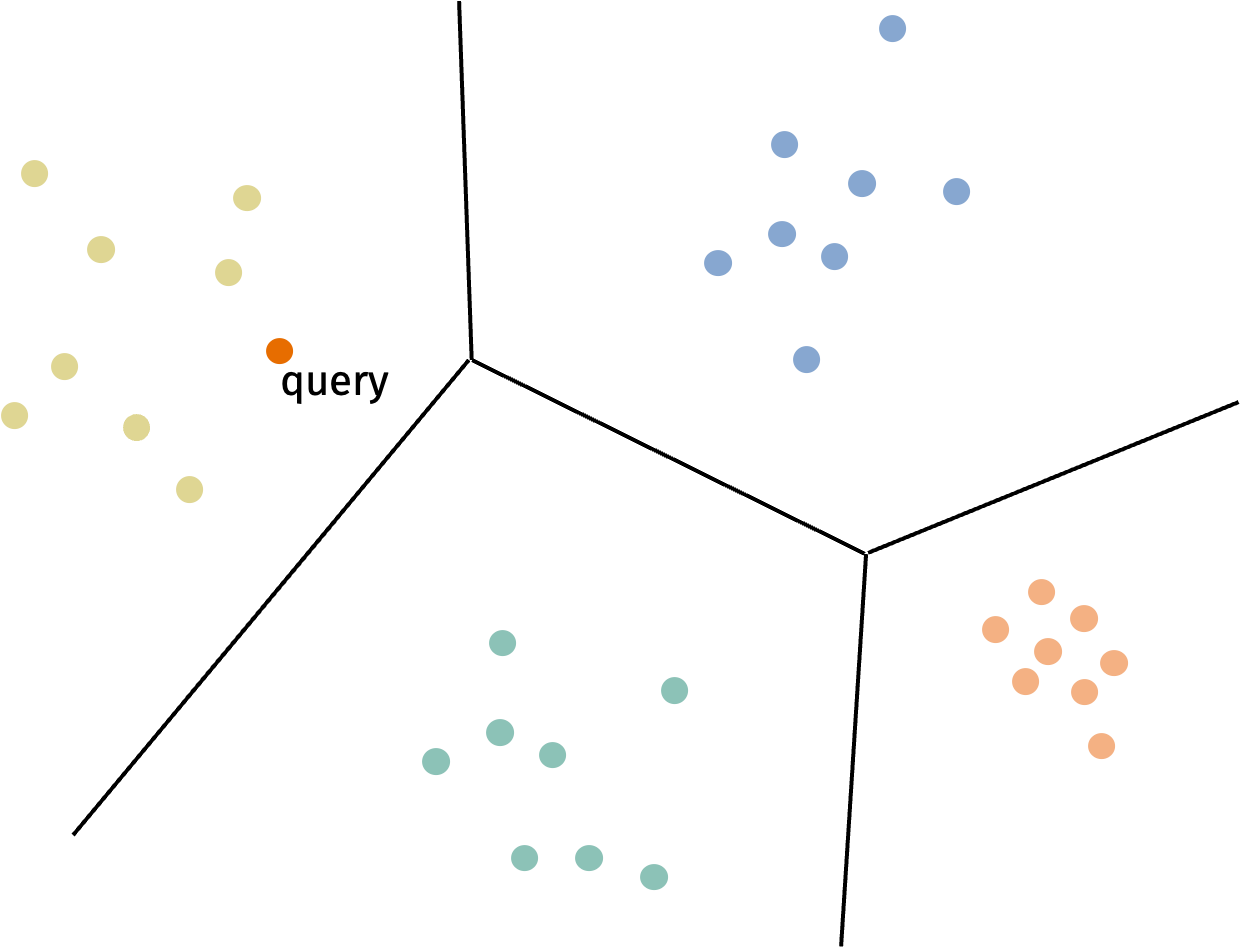
\includegraphics[width=.6\textwidth]{kmeans_1.png}
	\end{center}

\end{frame}

\begin{frame}[t]
	\frametitle{nearest-neighbor search in practice}
	\textbf{Common approach:} Split data using $k$-means clustering. 
	\begin{center}
	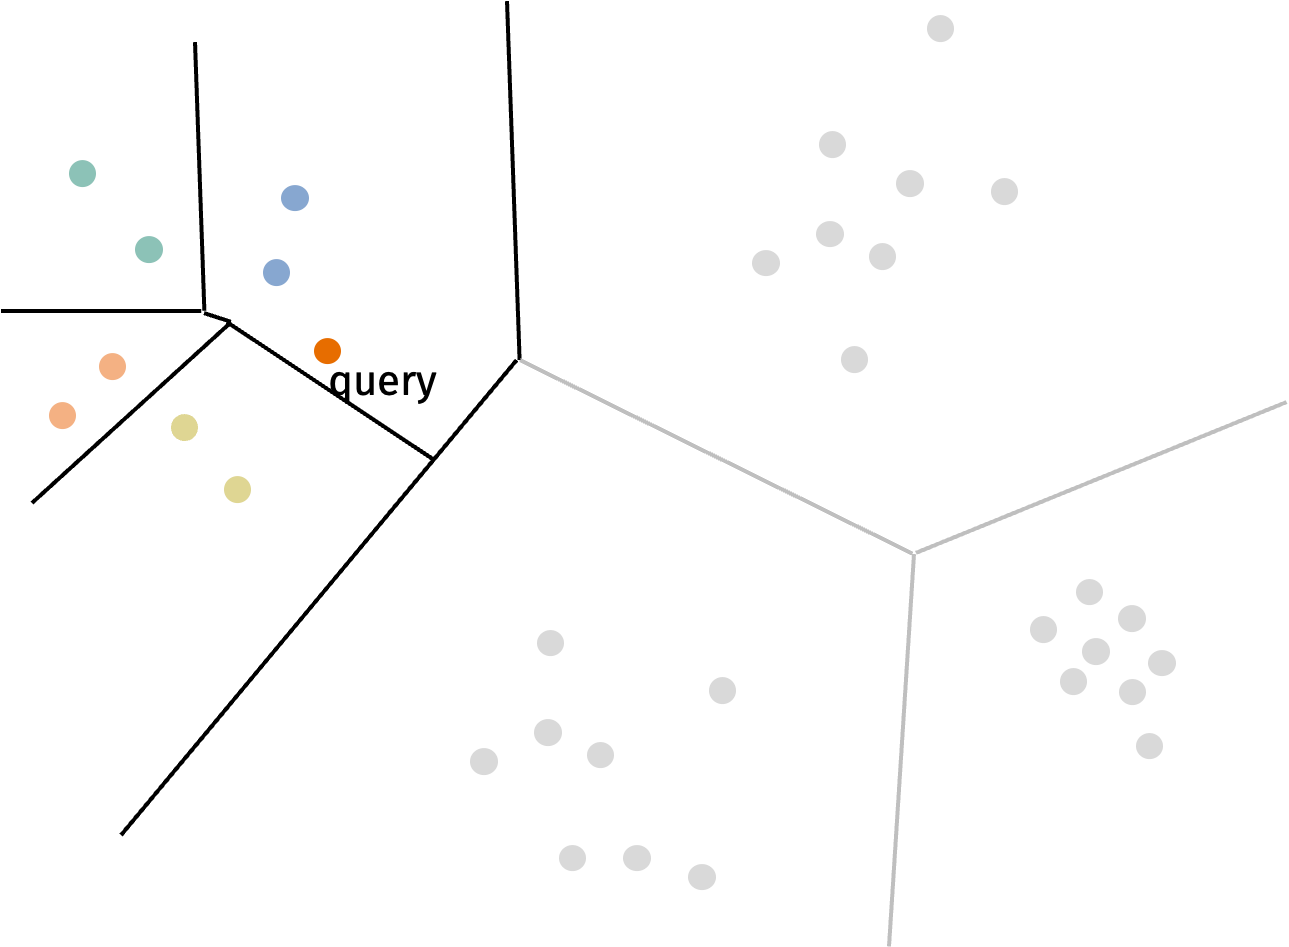
\includegraphics[width=.6\textwidth]{kmeans_2.png}
	\end{center}
	Main approach behind ``k-means tree'' and ``inverted file index'' based near-neighbor search methods like Meta's FAISS library and Google's SCANN. 
\end{frame}

\begin{frame}[t]
	\frametitle{nearest-neighbor search in practice}
	\textbf{New kid on the block:} Graph-based nearest neighbor search.
	\begin{center}
		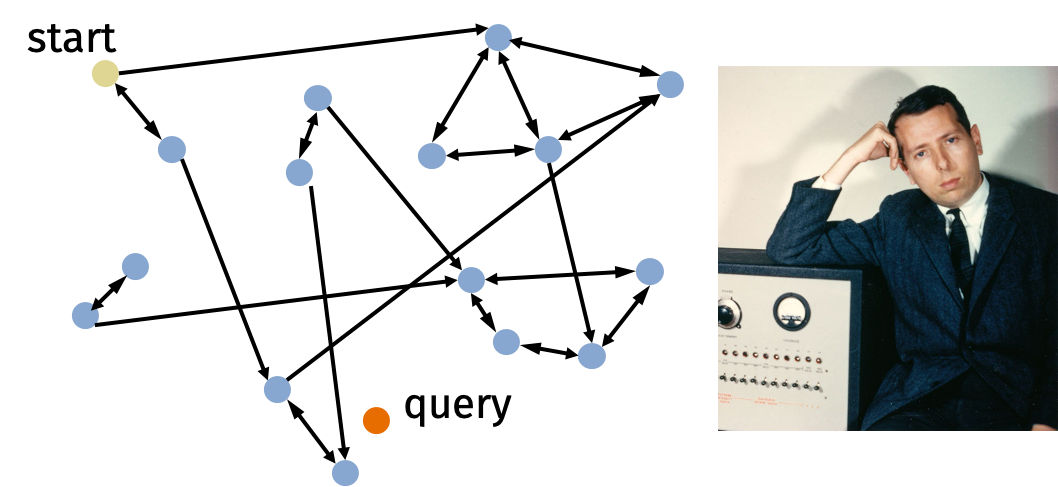
\includegraphics[width=\textwidth]{search_graph.png}
		\end{center}
Idea behind methods like NSG, HNSW, DiskANN, etc. Inspired by Milgram's famous ``small-world'' experiments from the 1960's. 
\end{frame}

\begin{frame}[t]
	\frametitle{open theory challenge}
	\textbf{Can we better explain the success of data-dependent nearest-neighbor search methods?}
	\begin{center}
		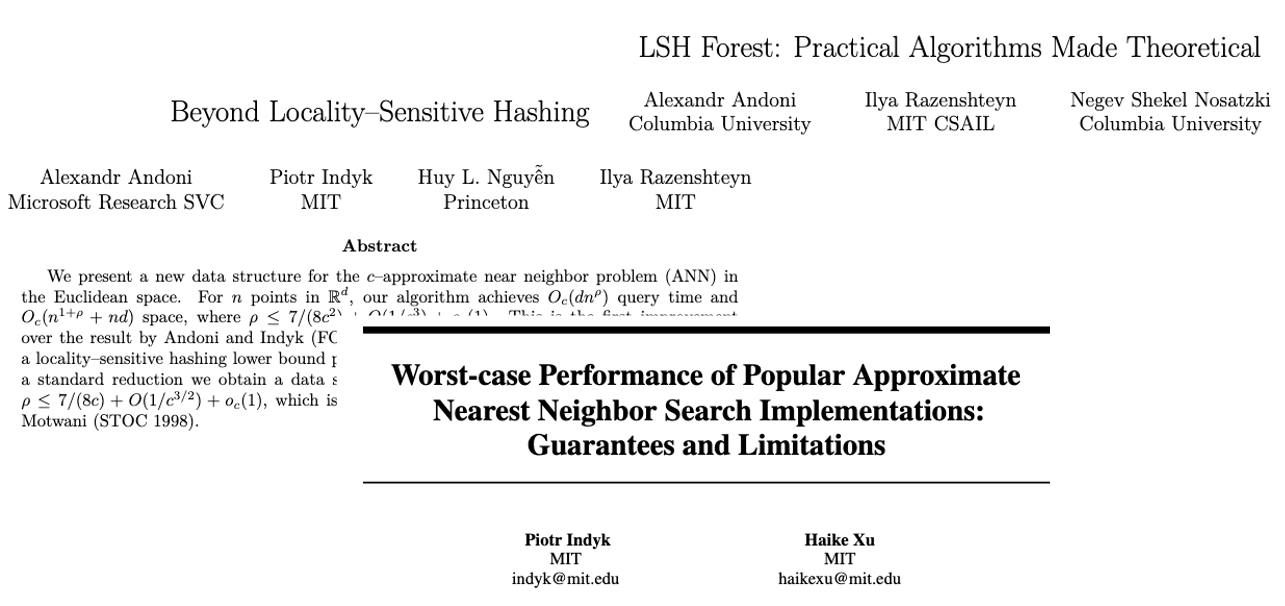
\includegraphics[width=\textwidth]{new_theory.png}
	\end{center}
\end{frame}

% \begin{frame}[t]
% 	\frametitle{modern near neigbhor search}
% 	\begin{itemize}
% 		\item High-dimensional vector search is exploding as a research area with the rise of machine-learned multi-modal embeddings for images, text, and more. 
% 	\end{itemize}
% 	\begin{center}
% 		\vspace{-.5em}
% 				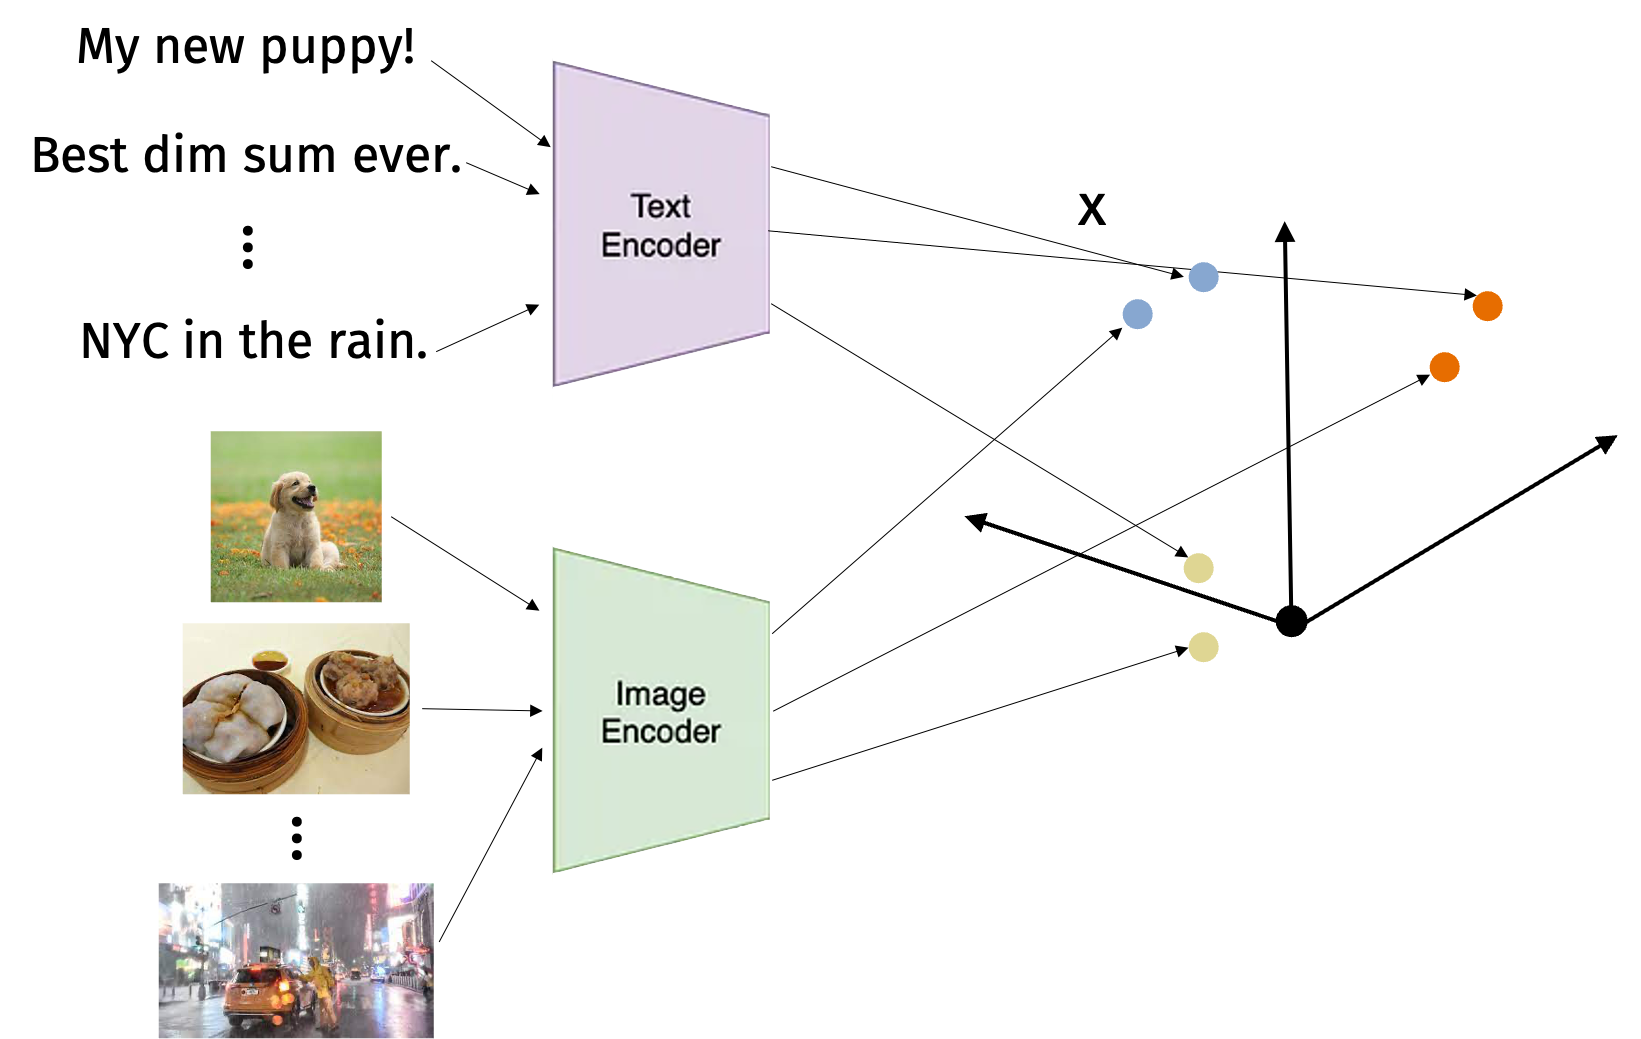
\includegraphics[width=.8\textwidth]{multimodal_embeddings.png}
% 				\vspace{-.5em}
% 	\end{center}
% 	Web-scale image search is now a vector search problem. 
% \end{frame}

% \begin{frame}[t]
% 	\frametitle{graph based near neigbhor}
	
% \end{frame}


\end{document} 








